% =====================================================================
%  PROYECTO DE TÍTULO — Archivo principal ("timeline master")
%  Ingeniería Civil · Universidad Católica del Maule · ICV-611
%  Compilar desde la raíz del repo con:  make pdf
%  Este archivo solo ARMA la tesis: no escribir contenido aquí.
%  Orden y formato según 01_normativa/REGLAS_FORMATO.md
% =====================================================================
\documentclass[12pt, letterpaper, oneside]{report}

%TC:ignore  (texcount: no contar la configuración)
% =====================================================================
%  Paquetes. Cada uno con un comentario de para qué sirve.
% =====================================================================

% --- Idioma y codificación ---
\usepackage[T1]{fontenc}
\usepackage[utf8]{inputenc}
% es-tabla: "Tabla" en vez de "Cuadro"; es-noshorthands evita conflictos con TikZ
\usepackage[english, spanish, es-tabla, es-noshorthands, es-lcroman]{babel} % el último idioma es el principal
\usepackage{csquotes}           % comillas correctas con \enquote{...}

% --- Fuente (provisoria; cambiar según normativa) ---
\usepackage{lmodern}
% Alternativas tipo Times o Arial (descomentar UNA):
% \usepackage{newtxtext,newtxmath}   % parecida a Times New Roman
% \usepackage[scaled]{helvet}\renewcommand{\familydefault}{\sfdefault} % parecida a Arial

% --- Matemática ---
\usepackage{amsmath, amssymb, mathtools}
\usepackage{bm}                 % vectores/matrices en negrita: \bm{u}
\usepackage{icomma}             % coma decimal sin espacio extra en modo matemático

% --- Unidades (fundamental en ingeniería) ---
\usepackage{siunitx}
\sisetup{
  output-decimal-marker = {,},  % coma decimal (estilo español)
  group-separator = {.},
  group-minimum-digits = 4,
  per-mode = symbol,            % kN/m en vez de kN m^-1
  range-phrase = { a },
  list-final-separator = { y },
}

% --- Figuras, tablas y diagramas ---
\usepackage{graphicx}
\usepackage{booktabs}           % tablas profesionales (\toprule, \midrule, \bottomrule)
\usepackage{tabularx}
\usepackage{multirow}
\usepackage{longtable}          % tablas de varias páginas
\usepackage{caption}
\usepackage{subcaption}         % subfiguras (a), (b)
\usepackage{float}
\usepackage{tikz}               % diagramas dibujados con código
\usetikzlibrary{arrows.meta, positioning, calc, patterns, decorations.pathmorphing, shapes.geometric}
\usepackage{pgfplots}           % gráficos con código
\pgfplotsset{compat=1.18}

% --- Listas, colores, varios ---
\usepackage{enumitem}
\usepackage{xcolor}
\usepackage{setspace}           % interlineado
\usepackage{geometry}           % márgenes
\usepackage{fancyhdr}           % encabezados y pies
\usepackage{titlesec}           % formato de títulos
\usepackage{pdfpages}           % insertar PDFs (p.ej. hoja oficial firmada)
\usepackage{listings}           % código fuente en anexos

% --- Bibliografía ---
% Estilo provisorio APA. Para IEEE: style=ieee. Para numérico simple: style=numeric-comp
\usepackage[backend=biber, style=apa]{biblatex}

% --- Enlaces y referencias cruzadas (cargar al final) ---
\usepackage[hidelinks]{hyperref}
\usepackage[spanish, noabbrev]{cleveref}   % \cref{fig:x} -> "figura 2.1"
   % paquetes
% =====================================================================
%  Formato de página según la normativa ICV-611 (UCM).
%  Cada bloque indica la regla de 01_normativa/REGLAS_FORMATO.md que aplica.
%  LIN = Lineamientos (§6), TPL = template Word oficial.
% =====================================================================

% --- Márgenes: sup 2,5 / inf 2,5 / izq 3 / der 3 cm [§1, LIN] ---
% El encabezado y el número de página quedan DENTRO del margen (como en TPL).
\geometry{
  top        = 2.5cm,
  bottom     = 2.5cm,
  left       = 3cm,
  right      = 3cm,
  headheight = 15pt,
  headsep    = 0.85cm,
  footskip   = 1.2cm,
}

% --- Interlineado 1,5 [§1, LIN] ---
% "1,5 líneas" de Word con Times 12 = 20,7 pt entre líneas. En LaTeX eso es
% \setstretch{1.43} (el \onehalfspacing de LaTeX es más estrecho, ~18 pt, y
% haría que la tesis ocupe menos páginas que su equivalente en Word).
\setstretch{1.43}

% --- Párrafos: justificado, sangría 1,25 cm, sin espacio extra [§1, TPL] ---
\setlength{\parindent}{1.25cm}
\setlength{\parskip}{0pt}

% --- Numeración y encabezados [§2, LIN + TPL] ---
% Número: abajo a la derecha, solo el número.
% Encabezado: arriba a la derecha "Capítulo N. Nombre"; en anexos "Anexos".
% Sin líneas ni leyendas extra.
\renewcommand{\headrulewidth}{0pt}
\renewcommand{\footrulewidth}{0pt}
\fancypagestyle{cuerpo}{%
  \fancyhf{}%
  \fancyhead[R]{\nouppercase{\leftmark}}%
  \fancyfoot[R]{\thepage}%
}
\fancypagestyle{plain}{%  primera página de cada capítulo y preliminares: solo número
  \fancyhf{}%
  \fancyfoot[R]{\thepage}%
}
\renewcommand{\chaptermark}[1]{\markboth{Capítulo~\thechapter.~#1}{}}
\renewcommand{\sectionmark}[1]{}
\pagestyle{plain}

% --- Títulos [§5, TPL] ---
% Capítulo: "1. Introducción y Planteamiento del Problema", 18 pt negrita, izquierda
\titleformat{\chapter}[hang]
  {\normalfont\fontsize{18}{22}\selectfont\bfseries\raggedright}
  {\thechapter.}{0.5em}{}
% Títulos sin número (Resumen, Índice General, Glosario, Bibliografía...): igual, sin número
\titleformat{name=\chapter, numberless}[hang]
  {\normalfont\fontsize{18}{22}\selectfont\bfseries\raggedright}
  {}{0pt}{}
\titlespacing*{\chapter}{0pt}{0pt}{30pt}
% Sección: "1.1. Título", 14 pt negrita
\titleformat{\section}
  {\normalfont\fontsize{14}{17}\selectfont\bfseries\raggedright}
  {\thesection.}{1em}{}
\titlespacing*{\section}{0pt}{12pt}{3pt}
% Subsección: "1.1.1. Título", 12 pt negrita
\titleformat{\subsection}
  {\normalfont\normalsize\bfseries\raggedright}
  {\thesubsection.}{1em}{}
\titlespacing*{\subsection}{0pt}{12pt}{3pt}
% Máximo 3 niveles numerados (1.1.1) [LIN]
\setcounter{secnumdepth}{2}
\setcounter{tocdepth}{1}       % Índice General: capítulos y secciones (como TPL)

% --- Índices (tocloft) [§3, §5, TPL] ---
\renewcommand{\cftchapfont}{\normalfont}
\renewcommand{\cftchappagefont}{\normalfont}
\renewcommand{\cftchapleader}{\cftdotfill{\cftdotsep}}
\renewcommand{\cftchapaftersnum}{.}
\renewcommand{\cftsecaftersnum}{.}
\setlength{\cftbeforechapskip}{4pt}
\setlength{\cftsecindent}{1.25cm}
\setlength{\cftsecnumwidth}{3em}
% Índice de Figuras / Tablas: "Figura 1.1: Título ....... 11"
\renewcommand{\cftfigpresnum}{Figura~}
\renewcommand{\cftfigaftersnum}{:}
\renewcommand{\cfttabpresnum}{Tabla~}
\renewcommand{\cfttabaftersnum}{:}
\setlength{\cftfigindent}{0pt}
\setlength{\cfttabindent}{0pt}
\setlength{\cftfignumwidth}{6.2em}
\setlength{\cfttabnumwidth}{5.8em}
% Rótulo "Pág." sobre la columna de números (se escribe al inicio de cada índice)
\newcommand{\rotulopag}{\protect\hfill\protect\textbf{Pág.}\protect\par}

% --- Leyendas: 11 pt, negrita solo en el rótulo, "Figura 2.2: Título" [§6, LIN] ---
% Tablas: título ARRIBA. Figuras: título ABAJO.
\DeclareCaptionFont{simple}{\setstretch{1.1}}
\captionsetup{font={small,simple}, labelfont=bf, textfont=normalfont,
  labelsep=colon, justification=centering, skip=6pt}
\captionsetup[table]{position=above}
\captionsetup[figure]{position=below}
% Contenido de las tablas también en 11 pt [§6, LIN]
\AtBeginEnvironment{table}{\small\setstretch{1.15}}
\AtBeginEnvironment{longtable}{\small\setstretch{1.15}}

% --- Numeración por capítulo: ecuaciones (1.1), figuras 1.1, tablas 1.1 [§6] ---
\numberwithin{equation}{chapter}

% --- Anexos: "Anexo I: Título", secciones "I.1.", encabezado "Anexos" [§5, TPL] ---
\newcommand{\iniciaranexos}{%
  \cleardoublepage
  \markboth{Anexos}{Anexos}%
  \chapter*{Anexos}%
  \thispagestyle{cuerpo}%
  \addcontentsline{toc}{chapter}{Anexos}%
  \appendix
  \renewcommand{\thechapter}{\Roman{chapter}}%
  \titleformat{\chapter}[hang]
    {\normalfont\fontsize{18}{22}\selectfont\bfseries\raggedright}
    {\appendixname~\thechapter:}{0.4em}{}%
  \renewcommand{\chaptermark}[1]{\markboth{Anexos}{Anexos}}%
  \assignpagestyle{\chapter}{cuerpo}% en TPL los anexos llevan "Anexos" también en su 1.ª página
  % el formato del índice se escribe DENTRO del .toc para que aplique solo a los anexos
  \addtocontents{toc}{\protect\renewcommand{\protect\cftchappresnum}{\appendixname~}}%
  \addtocontents{toc}{\protect\renewcommand{\protect\cftchapaftersnum}{:}}%
  \addtocontents{toc}{\protect\setlength{\protect\cftchapnumwidth}{5em}}%
}

% --- Bibliografía: título "Bibliografía", en el índice, encabezado "Bibliografía" ---
\defbibheading{bibliografia}{%
  \chapter*{Bibliografía}%
  \addcontentsline{toc}{chapter}{Bibliografía}%
  \markboth{Bibliografía}{Bibliografía}%
}
% Sangría francesa y separación entre referencias (APA)
\setlength{\bibitemsep}{0.5\baselineskip}

% --- Rutas ---
\graphicspath{{figuras/}}

% --- Estilo de código en anexos ---
\lstset{basicstyle=\ttfamily\small, breaklines=true, frame=single, numbers=left, numberstyle=\tiny}
    % márgenes, fuente, interlineado, títulos
% =====================================================================
%  Comandos propios y datos de la tesis (un solo lugar para cambiarlos)
% =====================================================================

% --- Datos de la tesis (se usan en portada, metadatos del PDF, etc.) ---
\newcommand{\tesisTitulo}{Título provisorio de la tesis}
\newcommand{\tesisAutor}{Marco Briones}
\newcommand{\tesisGrado}{Memoria para optar al título de Ingeniero Civil}
\newcommand{\tesisUniversidad}{Nombre de la Universidad}
\newcommand{\tesisFacultad}{Facultad de Ingeniería}
\newcommand{\tesisDepartamento}{Departamento de Ingeniería Civil}
\newcommand{\tesisGuia}{Nombre del Profesor Guía}
\newcommand{\tesisCiudad}{Ciudad}
\newcommand{\tesisAnio}{\the\year}

\hypersetup{pdftitle={\tesisTitulo}, pdfauthor={\tesisAutor}}

% --- Marcas de trabajo ---
% Para la versión final cambiar \mostrarmarcastrue por \mostrarmarcasfalse
\newif\ifmostrarmarcas
\mostrarmarcastrue
\ifmostrarmarcas
  \newcommand{\pendiente}[1]{\textcolor{red}{\textbf{\lbrack PENDIENTE:} #1\textbf{\rbrack}}}
  \newcommand{\revisar}[1]{\textcolor{orange}{\textbf{\lbrack REVISAR:} #1\textbf{\rbrack}}}
\else
  \newcommand{\pendiente}[1]{}
  \newcommand{\revisar}[1]{}
\fi

% --- Notación matemática (mantener consistente con 00_proyecto/GLOSARIO.md) ---
\newcommand{\vect}[1]{\bm{#1}}                 % vector
\newcommand{\matr}[1]{\mathbf{#1}}             % matriz
\newcommand{\dd}{\mathop{}\!\mathrm{d}}        % diferencial: \dd x
\newcommand{\deriv}[2]{\frac{\dd #1}{\dd #2}}  % derivada
\newcommand{\pderiv}[2]{\frac{\partial #1}{\partial #2}}
\newcommand{\fc}{f'_{c}}                       % resistencia del hormigón

% --- Unidades no estándar en siunitx ---
\DeclareSIUnit{\tonf}{tonf}
\DeclareSIUnit{\kgf}{kgf}

% --- Nombres en español: "Anexo" en vez de "Apéndice", "tabla" en vez de "cuadro" ---
\addto\captionsspanish{\renewcommand{\appendixname}{Anexo}}
\crefname{table}{tabla}{tablas}
\Crefname{table}{Tabla}{Tablas}
\crefname{appendix}{anexo}{anexos}
\Crefname{appendix}{Anexo}{Anexos}
\crefname{equation}{ecuación}{ecuaciones}
\Crefname{equation}{Ecuación}{Ecuaciones}
   % comandos propios y datos de la tesis
%TC:endignore

\addbibresource{bib/referencias.bib}

% Para compilar solo algunos capítulos mientras trabajas (más rápido),
% descomenta y ajusta la siguiente línea:
% \includeonly{capitulos/02_marco_teorico}

\begin{document}

% Rótulo "Pág." al inicio de cada índice (como en el template)
\addtocontents{toc}{\rotulopag}
\addtocontents{lof}{\rotulopag}
\addtocontents{lot}{\rotulopag}

% ---------- Portada y hoja de firmas (sin número de página) ----------
% =====================================================================
%  Portada — según template oficial ICV-611 (TPL p. 1) y Anexo 3 de los
%  Lineamientos. Los datos se editan en config/comandos.tex.
% =====================================================================
\begin{titlepage}
  \centering
  \setstretch{1}
  \fontsize{12}{14}\selectfont
  
\includegraphics[width=2.4cm]{portada/logo_ucm.png}\par
  \vspace{1.2cm}
  \MakeUppercase{\tesisUniversidad}\par
  \MakeUppercase{\tesisFacultad}\par
  \MakeUppercase{\tesisEscuela}\par
  \vspace{2.2cm}
  {\fontsize{14}{17}\selectfont\bfseries\MakeUppercase{\tesisTitulo}\par}
  \vspace{2cm}
  {\bfseries\MakeUppercase{\tesisAutor}\par}
  \vspace{0.3cm}
  {\bfseries PROFESOR GUÍA: \MakeUppercase{\tesisGuia}\par} % chktex 13
  \ifx\tesisCoGuia\empty\else\vspace{0.2cm}{\bfseries PROFESOR CO-GUÍA: \MakeUppercase{\tesisCoGuia}\par}\fi % chktex 13
  \vfill
  Proyecto de Título presentado en conformidad a los\par
  requisitos para obtener el título de \tesisTituloProfesional\par
  \vspace{1cm}
  \MakeUppercase{\tesisCiudad}, \tesisFecha\par
\end{titlepage}

% =====================================================================
%  Hoja de firmas Comisión Examinadora — según template oficial (TPL p. 2)
%  y Anexo 4 de los Lineamientos. Datos en config/comandos.tex.
%  Si se entrega la hoja firmada escaneada, reemplazar todo por:
%  \includepdf{portada/hoja_firmas_firmada.pdf}
% =====================================================================
\begin{titlepage}
  \centering
  \setstretch{1}
  \fontsize{12}{14}\selectfont
  
\includegraphics[width=2.4cm]{portada/logo_ucm.png}\par
  \vspace{1.2cm}
  \MakeUppercase{\tesisUniversidad}\par
  \MakeUppercase{\tesisFacultad}\par
  \MakeUppercase{\tesisEscuela}\par
  \vspace{1.2cm}
  Proyecto de título presentado en conformidad a los\par
  requisitos para obtener el título de \tesisTituloProfesional\par
  \vspace{1.2cm}
  {\fontsize{14}{17}\selectfont\bfseries\MakeUppercase{\tesisTitulo}\par}
  \vspace{1.2cm}
  {\bfseries\MakeUppercase{\tesisAutor}\par}
  \vspace{0.3cm}
  {\bfseries PROFESOR GUÍA: \MakeUppercase{\tesisGuia}\par} % chktex 13
  \ifx\tesisCoGuia\empty\else\vspace{0.2cm}{\bfseries PROFESOR CO-GUÍA: \MakeUppercase{\tesisCoGuia}\par}\fi % chktex 13
  \vspace{2.2cm}
  \renewcommand{\arraystretch}{2.4}
  \begin{tabular}{@{}p{5.6cm}@{\hspace{0.2cm}}l@{\hspace{0.3cm}}c@{}}
    & \textbf{COMISIÓN EXAMINADORA} & \textbf{FIRMA} \\
    \comisionGuia & PROFESOR GUÍA        & \rule{3.6cm}{0.4pt} \\
    \comisionDos  & PROFESOR DE COMISIÓN & \rule{3.6cm}{0.4pt} \\
    \comisionTres & PROFESOR DE COMISIÓN & \rule{3.6cm}{0.4pt} \\
  \end{tabular}
  \vfill
  \MakeUppercase{\tesisCiudad}, \tesisFecha\par
\end{titlepage}


% ---------- Preliminares (numeración romana: I, II, III...) ----------
\pagenumbering{Roman}
\pagestyle{plain}
% Agradecimientos — OPCIONAL, máximo 1 página [REGLAS_FORMATO §3]. Origen: v3.0.
\chapter*{Agradecimientos}
\addcontentsline{toc}{chapter}{Agradecimientos}
\label{pag:agradecimientos-ini}

Quisiera expresar mi más profundo agradecimiento a mi familia, cuyo apoyo incondicional, esfuerzo y paciencia han sido el pilar fundamental a lo largo de todos mis años de formación.

Agradezco sinceramente a mi profesor guía por la oportunidad brindada, su constante orientación y la confianza depositada en mí para llevar a cabo este desafío.

Asimismo, extiendo mi gratitud a la Agencia Nacional de Investigación y Desarrollo (ANID), ya que este trabajo se enmarca y fundamenta en la fase inicial del proyecto científico financiado ANID/Anillos/ATE250033, titulado \textit{\enquote{Nature-based solution strategies for developing new sustainable water sources in sweet cherry production under a scarcity context (NbS-Waterry)}}.

Finalmente, muchas gracias a todos quienes me apoyaron, directa o indirectamente, para hacer posible la culminación de esta etapa.
\label{pag:agradecimientos-fin}
   % opcional (máx. 1 página): comentar si no se usa
% Resumen — máx. 1 PÁGINA [REGLAS_FORMATO §3, RUBRICA "Resumen / Abstract" 5 %].
% Debe contener: contexto, objetivos, metodología, resultados CON DATOS CUANTITATIVOS
% y conclusiones. Luego, entre 3 y 5 palabras o expresiones clave.
% Origen: v3.0 (2026-11-19), citas migradas a biblatex.
\chapter*{Resumen}
\addcontentsline{toc}{chapter}{Resumen}
\label{pag:resumen-ini}

% Estructura pedida por el profesor guía (16-11-2026): 4 párrafos.
% (1) introductorio · (2) objetivo general + algo de metodología · (3) resultados · (4) síntesis de conclusiones.

La Región del Maule enfrenta una creciente escasez hídrica que afecta a la producción agrícola, por lo que la reutilización de aguas residuales tratadas para riego surge como una fuente alternativa de agua.
En zonas rurales, los sistemas de tratamiento convencionales resultan complejos de implementar, mientras que las Soluciones Basadas en la Naturaleza, como los humedales construidos, ofrecen una alternativa descentralizada y de baja demanda energética.
En este contexto, el proyecto ANID/Anillos/ATE250033 contempla una estación experimental para tratar tres fuentes de agua residual de un predio frutícola de la Región del Maule: aguas servidas domésticas, aguas de lavado de agroquímicos y agua del estero Batuco.

El objetivo de este trabajo fue diseñar un sistema experimental de humedales construidos de flujo vertical para el tratamiento de esas tres fuentes y su futura reutilización en riego, integrando el sistema hidráulico y las necesidades estructurales para su implementación.
Para ello se caracterizaron las fuentes mediante seis campañas de muestreo en cinco puntos; se dimensionaron los humedales con el método del balance de oxígeno; se calcularon las redes por gravedad y las líneas a presión con la ecuación de Hazen-Williams; y se diseñaron los elementos de soporte con el método LRFD y el análisis sísmico de la NCh2369.

\pendiente{Párrafo de resultados con cifras: DQO y nitrógeno de cada fuente; caudal de la línea doméstica (\qty{0.75}{\cubic\meter\per\day}); \qty{6}{\square\meter} por línea en 6 IBC, con \qty{315}{\gram\per\day} de oxígeno frente a una demanda de \qty{111.8}{\gram\per\day}; ADT y bombas; perfiles de la plataforma y presión de contacto (cuando resuelva las preguntas al profesor).}

\pendiente{Párrafo de conclusiones en 3--4 oraciones: factibilidad del diseño, condiciones críticas (horizontalidad de la plataforma, impulsión del estero) y uso del expediente para construir la estación.}

\noindent\textbf{Palabras clave:} Humedales Construidos, Soluciones Basadas en la Naturaleza, Diseño Hidráulico, Cálculo Estructural.
\label{pag:resumen-fin}
           % máx. 1 página, 3 a 5 palabras clave
% Abstract — traducción al inglés del Resumen + keywords [REGLAS_FORMATO §3]
% Traducción del Resumen de la versión 4 (20-11-2026). Actualizar cuando se actualice el Resumen.
\chapter*{Abstract}
\addcontentsline{toc}{chapter}{Abstract}
\begin{otherlanguage}{english}
The Maule Region faces growing water scarcity that affects agricultural production, and the reuse of treated wastewater for irrigation is emerging as an alternative water source; in rural areas, constructed wetlands, a Nature-based Solution, offer a decentralized, low-energy alternative.
In this context, the ANID/Anillos/ATE250033 project includes an experimental station to treat three sources from a fruit farm: domestic wastewater, agrochemical washing water and water from the Batuco stream.

The objective of this work was to design an experimental system of vertical-flow constructed wetlands for these three sources, integrating the hydraulic system and the structural requirements for its implementation.
The sources were characterized in six sampling campaigns, the wetlands were sized with the oxygen balance method, the pipelines were calculated with the Hazen-Williams equation, and the supporting elements were designed with the LRFD method and the Chilean seismic standard NCh2369.

Office wastewater showed a mean COD of \qty{411}{\milli\gram\per\liter}; agrochemical washing water, 76 to \qty{393}{\milli\gram\per\liter}; and stream water, \qty{6.3}{\milli\gram\per\liter}, but with class~4 microbiological contamination.
Each line treats \qty{750}{\liter\per\day} in six IBC containers (\qty{125}{\milli\meter\per\day}); in the domestic line, with \qty{30}{\gram\per\square\meter\per\day} of COD, the oxygen supply (\qty{315}{\gram\per\day}) nearly triples the demand (\qty{111.8}{\gram\per\day}).
A single \qty{0.55}{\kilo\watt} pump fills the \qty{1000}{\liter} tanks in 17 to \qty{36}{\minute}, and the steel platform meets the LRFD checks, with at least \qty{95}{\percent} of the footing area in contact under the design earthquake.

The design is technically feasible and documented for the construction of the station; its critical conditions are the continuity of the platform deck and its fastening as a diaphragm, the rigidity of the welded joints, and the assumed soil, which must be verified with a geotechnical study.

\noindent\textbf{Keywords:} Constructed wetlands, Nature-based Solutions, Hydraulic design, Structural calculation.
\end{otherlanguage}


\cleardoublepage\phantomsection\addcontentsline{toc}{chapter}{\contentsname}
\tableofcontents
\cleardoublepage\phantomsection\addcontentsline{toc}{chapter}{\listfigurename}
\listoffigures
\cleardoublepage\phantomsection\addcontentsline{toc}{chapter}{\listtablename}
\listoftables
% Glosario — términos técnicos y siglas [REGLAS_FORMATO §3]. Origen: v3.0.
% Mantener sincronizado con 00_proyecto/GLOSARIO.md. Orden alfabético.
\chapter*{Glosario}
\addcontentsline{toc}{chapter}{Glosario}

\begin{glosario}
  \item[ACV] Análisis de Ciclo de Vida.
  \item[ADT] Altura Dinámica Total. Energía requerida por un sistema de bombeo para transportar un fluido.
  \item[AGR1] Punto de muestreo correspondiente a los residuos agroquímicos generados en la bodega.
  \item[AGR2] Punto de muestreo correspondiente a los residuos agroquímicos captados en la sala de bombas.
  \item[ANID] Agencia Nacional de Investigación y Desarrollo.
  \item[AS1] Punto de muestreo correspondiente a las aguas servidas provenientes del sector de oficinas.
  \item[AS2] Punto de muestreo correspondiente a las aguas servidas habitacionales provenientes de la casa.
  \item[ASD] Diseño por Tensiones Admisibles (\textit{Allowable Stress Design}).
  \item[DBO$_5$] Demanda Bioquímica de Oxígeno medida a los cinco días.
  \item[DGA] Dirección General de Aguas.
  \item[DOH] Dirección de Obras Hidráulicas.
  \item[DQO] Demanda Química de Oxígeno.
  \item[EETT] Especificaciones Técnicas.
  \item[EST] Aguas del estero Batuco.
  \item[HC] Humedal Construido.
  \item[HC-FV] Humedal Construido de Flujo Subsuperficial Vertical.
  \item[IBC] Contenedor Intermedio para Graneles (\textit{Intermediate Bulk Container}).
  \item[INN] Instituto Nacional de Normalización.
  \item[LRFD] Diseño por Factores de Carga y Resistencia (\textit{Load and Resistance Factor Design}).
  \item[NMP] Número Más Probable (recuento de coliformes).
  \item[NT] Nitrógeno Total.
  \item[NTK] Nitrógeno Total Kjeldahl. Suma del nitrógeno orgánico y amoniacal.
  \item[OD] Demanda de Oxígeno del lecho filtrante (método del balance de oxígeno de Platzer). El oxígeno disuelto se escribe sin sigla.
  \item[OI] Aporte de Oxígeno al lecho filtrante.
  \item[PEAD] Polietileno de Alta Densidad.
  \item[PT] Fósforo Total.
  \item[PVC] Policloruro de Vinilo.
  \item[SbN] Soluciones Basadas en la Naturaleza.
  \item[SST] Sólidos Suspendidos Totales.
  \item[TRH] Tiempo de Retención Hidráulica.
\end{glosario}
          % si corresponde

% ---------- Cuerpo principal (numeración arábiga desde la Introducción) ----------
\cleardoublepage
\pagenumbering{arabic}
\pagestyle{cuerpo}
% =====================================================================
%  Capítulo 1: Introducción y Planteamiento del Problema
%  Rúbrica: 10 %. Debe actualizarse respecto al anteproyecto.
%  Exigido (LIN §6): contexto, antecedentes generales y técnicos, hipótesis
%  y/o preguntas de investigación, objetivos, contribuciones del proyecto.
%  Origen: v3.0 (2026-11-19). Ver 03_seleccion/triaje/2026-11-19_triaje_proyecto-titulo-v3.0.md
%  Tercera persona. Una oración por línea. Unidades con siunitx.
% =====================================================================
\chapter{Introducción y Planteamiento del Problema}
\label{cap:introduccion}

\section{Descripción del problema}
\label{sec:problema}

La Región del Maule enfrenta una severa y creciente vulnerabilidad hídrica derivada de las alteraciones del ciclo hidrológico y de prolongados eventos de sequía asociados al cambio climático~\parencite{uribe2012atlas}.
Esta situación amenaza directamente la sostenibilidad y competitividad de la producción agrícola, de manera particular el cultivo del cerezo dulce (\textit{Prunus avium} L.), una especie que ha experimentado una expansión acelerada en la zona durante el último lustro y que demanda volúmenes considerables de agua para su óptimo desarrollo~\parencite{allen1998crop}.
\revisar{La rúbrica pide justificar con datos cuantitativos y literatura actualizada: agregar cifras de déficit hídrico, superficie de cerezos en el Maule y una fuente reciente sobre la megasequía (p.\ ej.\ Garreaud et al., 2017 o 2020, verificar antes de citar).}

Ante la progresiva disminución en la disponibilidad de los recursos hídricos superficiales y subterráneos, resulta imperativo explorar y diversificar las fuentes de abastecimiento mediante la reutilización de aguas residuales tratadas.
No obstante, en zonas rurales y agrícolas descentralizadas, la implementación de sistemas de tratamiento convencionales (como lodos activados) resulta habitualmente inviable debido a sus altos costos de inversión, requerimientos energéticos y complejidad operativa~\parencite{tchobanoglous2014wastewater}.

En consecuencia, el problema a resolver consiste en la necesidad de diseñar e implementar tecnologías de depuración descentralizadas, eficientes y sostenibles ---específicamente mediante Soluciones Basadas en la Naturaleza (SbN)--- que sean capaces de tratar simultáneamente efluentes de distinta naturaleza (aguas servidas domésticas, riles de lavado de agroquímicos y aguas superficiales contaminadas).
El desafío de ingeniería radica en adaptar los modelos teóricos e hidráulicos de los humedales construidos a las solicitaciones reales de un entorno agrícola, garantizando que el efluente final cumpla con la normativa chilena de calidad para el riego agrícola y asegurando la estabilidad estructural del sistema en las instalaciones de Frutícola SABA SpA.

\section{Antecedentes}
\label{sec:antecedentes}

El desarrollo del presente proyecto de título se enmarca y fundamenta en la fase inicial de ingeniería del proyecto científico financiado por la Agencia Nacional de Investigación y Desarrollo, ANID/Anillos/ATE250033, titulado \textit{\enquote{Nature-based solution strategies for developing new sustainable water sources in sweet cherry production under a scarcity context (NbS-Waterry)}}.

Mientras que el proyecto marco contempla una investigación multidisciplinaria de tres años enfocada en evaluar la fisiología vegetal del cerezo dulce (\textit{Prunus avium} L.), la inocuidad del fruto y el Análisis de Ciclo de Vida (ACV) derivado de la reutilización de efluentes tratados, el presente trabajo se delimita al diseño de la infraestructura hidráulica y estructural.

La necesidad de este desarrollo de ingeniería surge porque los modelos teóricos de depuración mediante Soluciones Basadas en la Naturaleza (SbN), documentados ampliamente en la literatura para el tratamiento de aguas~\parencite{dotro2017treatment}, requieren ser adaptados y materializados físicamente en un entorno agrícola real bajo las exigencias normativas chilenas~\parencite{inn1987nch1333}.
El propósito de este proyecto es transformar los requerimientos biológicos e hidráulicos del sistema en un expediente técnico a nivel de ejecución.
Esto contempla establecer las memorias de cálculo, las especificaciones técnicas de materiales y la planimetría normalizada que garantizarán la posterior construcción y desarrollo de la planta piloto experimental en los terrenos de Frutícola SABA SpA.

\revisar{Agregar antecedentes técnicos de Chile: cobertura de tratamiento rural (\textcite{vera2016humedales} reporta cobertura menor al 20~\% en zonas rurales) y estado del reúso para riego, con Vera-Puerto et al. (2022), \emph{Water}, 14(4), 627, \url{https://doi.org/10.3390/w14040627} (verificado; del profesor guía): reúso directo menor al 1~\% del caudal tratado.
Modelo de redacción problema → brecha → propuesta: 05\_ejemplos/fichas/2026\_ucm\_jove\_….md.}

\section{Preguntas de investigación}
\label{sec:preguntas}

\pendiente{Exigido por los Lineamientos (§6): formular la hipótesis y/o las preguntas que guían el diseño.
Por ejemplo: ¿qué área activa de HCFV en módulos IBC satisface el balance de oxígeno para los caudales y cargas de cada afluente?
¿Qué configuración estructural de la plataforma asegura la estabilidad y la horizontalidad requerida por los sifones bajo la demanda sísmica de la NCh2369?}

\section{Objetivos}
\label{sec:objetivos}

\subsection{Objetivo general}

Diseñar la infraestructura hidráulica y estructural de una estación experimental basada en Humedales Construidos de Flujo Subsuperficial Vertical (HCFV), orientada al tratamiento y posterior reutilización agrícola de tres afluentes residuales independientes en Frutícola SABA SpA, comuna de Linares.

\subsection{Objetivos específicos}

\begin{enumerate}
  \item Dimensionar el sistema de depuración y las redes de conducción a presión y gravedad, estableciendo el balance de oxígeno de los humedales, los requerimientos operativos de los equipos de impulsión y las especificaciones técnicas para las distintas fuentes de agua.
  \item Desarrollar la modelación y el cálculo estructural de la plataforma de acero y sus fundaciones bajo solicitaciones estáticas y sísmicas normativas, integrando la planimetría consolidada y los detalles constructivos de la estación.
\end{enumerate}

\revisar{Cada objetivo agrupa varias tareas. Evaluar con el profesor guía separarlos (p.\ ej.: caracterizar caudales y cargas; dimensionar los HCFV; diseñar redes e impulsión; diseñar plataforma y fundaciones; elaborar planimetría e itemizado), para que Resultados y Conclusiones respondan uno a uno.}

\section{Contribuciones del proyecto}
\label{sec:contribuciones}

\pendiente{Exigido por los Lineamientos (§6): indicar el aporte concreto del proyecto (p.\ ej.: expediente técnico a nivel de ejecución de la primera estación experimental multifuente del proyecto ANID; adaptación del método de Platzer a módulos IBC; base para los monitoreos del proyecto marco).}

\section{Alcances y limitaciones}
\label{sec:alcances}

\pendiente{Precisar qué incluye el diseño (líneas de tratamiento, redes, plataforma, fundaciones, planos, itemizado) y qué no (operación, monitoreo, evaluación agronómica y ACV, que corresponden al proyecto marco).}

% =====================================================================
%  Capítulo: Marco teórico
%  Estado: ver 00_proyecto/ESTADO.md
%  Una oración por línea. Unidades con siunitx. Citas solo de referencias.bib.
% =====================================================================
\chapter{Marco teórico}
\label{cap:marco-teorico}

\section{Conceptos fundamentales}
\pendiente{Definiciones y teoría base, con fuentes.}

\section{Estado del arte}
\pendiente{Qué se ha hecho antes; síntesis de las fichas de 03\_seleccion/fichas\_lectura.}

\section{Normativa aplicable}
\pendiente{Normas y códigos de diseño que rigen el problema.}


% =====================================================================
%  Capítulo: Metodología
%  Rúbrica: 20 % (el criterio de mayor peso). Título según tipo de proyecto: 'Materiales y Métodos' o 'Metodología'.
%  Estado: ver 00_proyecto/ESTADO.md · Rúbrica: 01_normativa/RUBRICA.md
%  Tercera persona. Una oración por línea. Unidades con siunitx.
%  Citas solo de referencias.bib. Figuras/tablas citadas ANTES de aparecer.
% =====================================================================
\chapter{Metodología}
\label{cap:metodologia}

\section{Enfoque general}
\pendiente{Diagrama de flujo de la metodología y su relación con cada objetivo específico.}

\section{Datos y casos de estudio}
\pendiente{Origen, tratamiento y supuestos de los datos.}

\section{Modelación y cálculos}
\pendiente{Modelo o aplicación: hipótesis, ecuaciones, software y cálculos.}

\section{Validación}
\pendiente{Cómo se verifica que los resultados son correctos.}

\section{Planificación y entregables}
\pendiente{Etapas, carta Gantt y entregables definidos.}


% =====================================================================
%  Capítulo: Desarrollo y resultados
%  Estado: ver 00_proyecto/ESTADO.md
%  Una oración por línea. Unidades con siunitx. Citas solo de referencias.bib.
% =====================================================================
\chapter{Desarrollo y resultados}
\label{cap:resultados}

\section{Resultados}
\pendiente{Figuras y tablas generadas desde 04\_analisis/scripts.}


% =====================================================================
%  Capítulo 5: Discusión y Análisis de Resultados
%  Rúbrica: 15 %. Consistente con el marco teórico; relación resultados –
%  metodología – objetivos; responder TODOS los objetivos.
%  Reestructurado 2026-11-20 según los objetivos aprobados (VF-V2):
%  OE1 caracterización, OE2 diseño depurativo e hidráulico, OE3 estructural.
% =====================================================================
\chapter{Discusión y Análisis de Resultados}
\label{cap:discusion}

\section{Características fisicoquímicas y de producción de las fuentes}
\label{sec:dis-caracterizacion}

Las tres fuentes estudiadas presentan características muy distintas entre sí, lo que justifica tratarlas en líneas independientes.
Las aguas servidas de las oficinas tienen una DQO media de \qty{411}{\milli\gram\per\liter}, dentro del rango informado para las aguas servidas rurales de Chile (\cref{tab:caracteristicas-tipicas})~\parencite{araya2014aguas}, por lo que su carga orgánica es representativa de este tipo de efluente; en cambio, de la casa queda un único dato válido, lo que impide caracterizarla y justifica usar los valores de diseño del proyecto.
Con esos valores, la carga orgánica de la línea doméstica es de \qty{30}{\gram\per\square\meter\per\day} de DQO, y con las concentraciones medidas varía entre unos 17 y \qty{33}{\gram\per\square\meter\per\day} (\cref{tab:validacion-cargas}), por lo que el valor de diseño queda validado.
El amonio medido (1,0 a \qty{1.8}{\milli\gram\per\liter}) queda uno a dos órdenes de magnitud bajo los valores habituales (6 a \qty{60}{\milli\gram\per\liter})~\parencite{araya2014aguas}, y el nitrógeno total no es consistente con el amonio y el nitrato, por lo que el nitrógeno medido no se usa como dato de diseño.
En las oficinas, este nitrógeno bajo se explicaría principalmente por la dilución con el agua del lavamanos y de la cocina; en la casa no tiene una causa confirmada, y como no se midió el caudal de cada artefacto ni la calidad antes y después de la fosa, no es posible afirmarla.

Las aguas de lavado de agroquímicos muestran una variabilidad alta: la DQO de la bodega (\qty{393}{\milli\gram\per\liter}) es cinco veces la de la sala de bombas (\qty{75.7}{\milli\gram\per\liter}), y ambas quedan en el extremo inferior del amplio intervalo reportado para aguas con plaguicidas (150 a \qty{33750}{\milli\gram\per\liter})~\parencite{saleh2020removal}.
Esta variabilidad es propia de un efluente que depende de qué producto se aplica y de cuánta agua se usa en cada lavado, y refuerza el carácter experimental de esa línea.
Además, el volumen de lavado de un predio típico es pequeño, del orden de 5000 a \qty{7000}{\liter} al año~\parencite{braul2018robust}, por lo que la producción real del predio condiciona el caudal que esta línea puede tratar.

El agua del estero Batuco tiene una carga orgánica muy baja y una conductividad eléctrica similar a la de los ríos de la cuenca del Maule~\parencite{dga2004volumen1}; su limitación para el riego es microbiológica, ya que sus coliformes totales la ubican en la clase~4 y su \textit{E.~coli} supera el límite de la clase~1 para coliformes fecales (\cref{tab:clases-calidad}).
Por lo tanto, en esta línea el humedal no se justifica por la remoción de materia orgánica, sino por la reducción de patógenos, para la cual los humedales verticales alcanzan de 2 a 4 unidades logarítmicas~\parencite{langergraber2021vertical}.
Esta eficiencia es teórica y deberá comprobarse durante la operación.

En cuanto a la producción, el caudal de la casa (\qty{0.60}{\cubic\meter\per\day}) se obtuvo de un registro de trece meses con un factor de restitución de \num{0.85}, en el extremo superior del rango de 60 a \qty{85}{\percent} informado en Chile~\parencite{vidal2023desarrollo}, lo que deja el dimensionamiento del lado de la seguridad.
El caudal de las oficinas (\qty{0.15}{\cubic\meter\per\day}) se apoya en solo un mes de registro de usos, por lo que es la estimación con mayor incertidumbre de la línea doméstica.
Para las líneas del estero y de agroquímicos se adoptó la misma carga hidráulica que en la línea doméstica (\qty{750}{\liter\per\day}), porque aplicarles la misma carga orgánica exigiría caudales inviables (unos \qty{28400}{\liter\per\day} en el estero).
Este criterio, coherente con el enfoque sanitario de la estación, hace que cada línea reciba una carga orgánica distinta: \qty{0.8}{\gram\per\square\meter\per\day} en el estero y entre 9,5 y \qty{49}{\gram\per\square\meter\per\day} en agroquímicos según la proporción de AGR1 y AGR2, por lo que en esta última conviene mezclar las fuentes, o completar con agua del estero, para que la DQO de la mezcla no supere unos \qty{240}{\milli\gram\per\liter}.
Como el volumen de lavado de un predio típico es pequeño, el agua del estero cumple además la función de completar el caudal de las otras líneas.

\section{Diseño depurativo y cálculo hidráulico}
\label{sec:dis-hidraulico}

El balance de oxígeno indica que el área activa de \qty{6.00}{\square\meter} por línea aporta \qty{315.0}{\gram\per\day} de O$_2$ frente a una demanda de \qty{111.8}{\gram\per\day} (\cref{tab:balance-oxigeno}), de modo que el lecho puede operar en condiciones aerobias sin aireación forzada~\parencite{platzer1999design,dotro2021humedales}.
Este margen se debe en gran parte al nitrógeno bajo de las concentraciones de diseño: la nitrificación aporta solo \qty{4.7}{\gram\per\day} de la demanda, y con concentraciones de nitrógeno típicas de aguas servidas la demanda aumentaría de forma importante, por lo que el margen debe interpretarse con cautela.

La carga orgánica de \qty{30}{\gram\per\square\meter\per\day} de DQO y la carga hidráulica de \qty{125}{\milli\meter\per\day} superan los máximos de las guías europeas (20 a \qty{27}{\gram\per\square\meter\per\day} y \qty{80}{\liter\per\square\meter\per\day}, \cref{tab:parametros-hcfv}), pero esas guías se desarrollaron para climas con inviernos fríos~\parencite{dotro2021humedales}.
En climas cálidos se han aplicado hasta \qty{200}{\milli\meter\per\day} y \qty{32}{\gram\per\square\meter\per\day} de DBO$_5$~\parencite{platzer2016long}, y diseños recientes en Chile aceptan hasta \qty{35}{\gram\per\square\meter\per\day} de DQO~\parencite{vera2025atrapaniebla}, por lo que las cargas de la Fase~1 quedan dentro de la experiencia regional.
Estas cargas no responden a un criterio conservador, sino a la Fase~1 experimental del proyecto ANID/Anillos/ATE250033, que busca evaluar cuánta agua puede tratarse sin deteriorar la calidad del efluente; el riesgo de colmatación deberá vigilarse en la operación.
Además, los 6 pulsos diarios del balance de oxígeno implican un intervalo de \qty{4}{\hour} entre cargas, dentro del rango de 3 a \qty{6}{\hour} de la guía austríaca, pero menor que las \qty{6}{\hour} que recomienda la guía alemana~\parencite{dotro2021humedales}, por lo que el número de pulsos es un parámetro que convendrá ajustar en la operación.

La configuración en módulos IBC independientes separa físicamente las tres aguas, lo que evita la mezcla entre líneas y permite evaluar el desempeño de cada una por separado, y su instalación sobre el terreno evita excavaciones.
Este tipo de solución en estanques prefabricados es coherente con la experiencia piloto en humedales verticales construidos en recipientes de polietileno~\parencite{ignatowicz2023treatment}, y con la necesidad, señalada para Latinoamérica, de sistemas de distribución presurizada sencillos que faciliten la adopción de los humedales verticales~\parencite{rodriguezdominguez2020constructed}.

En la parte hidráulica, la línea del estero es la más exigente (\cref{tab:bombas-adt}): con PVC de \qty{25}{\milli\meter} en \qty{140}{\meter} y \qty{13.82}{\meter} de desnivel, no alcanza el llenado deseable de \qty{30}{\minute}, pero con la bomba periférica supuesta llena el estanque en unos \qty{36}{\minute}, dentro del límite de \qty{60}{\minute}, sin cambiar el diámetro especificado.
Usar la misma bomba en las tres líneas simplifica la operación y la mantención, porque permite intercambiarla ante una falla.
Por otra parte, el caudal del microrriego (\qty{160}{\liter\per\hour}, \cref{tab:demanda-riego}) es muy inferior al de estas bombas, por lo que requiere otro equipo o un circuito de retorno (\textit{bypass}).
Finalmente, como el trazado de las zanjas se definió en terreno, el diseño entrega los criterios de las zanjas y no su cubicación.

\section{Diseño y cálculo estructural}
\label{sec:dis-estructural}

Frente a las cargas gravitacionales, los perfiles cajón de la plataforma trabajan con razones de demanda a capacidad bajas (alrededor del \qty{9}{\percent} a flexión en la viga principal, \cref{tab:verificacion-estructural}).
Este margen no indica un sobredimensionamiento sin propósito: la condición que controla el diseño es la deformación, porque la plataforma debe mantener nivelados los estanques de almacenamiento y sus conexiones.
En ese sentido, el elemento crítico es el tablero de \qty{15}{\milli\meter}: modelado como un solo vano, no cumplía $L/300$, pero su condición real es la de una lámina continua sobre varias vigas, y con ese modelo cumple con una razón de \num{0.91}.
Como el margen es estrecho y el tablero no cumple la referencia de $L/500$ que la NCh427/1 sugiere para equipos~\parencite{inn2016nch427}, la continuidad de los paños bajo los estanques y el módulo de elasticidad real del tablero fenólico son condiciones del diseño.
Los sifones, en cambio, se ubican en los dosificadores sobre la estructura auxiliar, cuya flecha hace descender el estanque completo sin inclinarlo, aunque sus columnas esbeltas hacen que su estabilidad lateral dependa del arriostramiento y del anclaje.

Frente al sismo, la verificación depende más de cómo se reparte el corte entre los pilares y de la categoría de ocupación que de la versión de la norma (\cref{tab:sismo-zapatas}).
Si los dos pilares de un marco resisten el corte en voladizo, la zapata vuelca con las versiones de 2003 y de 2025; si el tablero y las vigas actúan como diafragma y los seis pilares comparten el corte, con la categoría~I y el suelo~C supuesto el área apoyada es del \qty{91}{\percent}, sobre el mínimo de \qty{80}{\percent} de la NCh2369:2025~\parencite{inn2025nch2369}.
Con la categoría~II el margen desaparece (76 a \qty{79}{\percent}), por lo que la elección de la categoría~I, propia de una estación experimental cuya falla no detiene ninguna operación ni pone en riesgo otras estructuras, es la que permite mantener las zapatas de \qty{1.0}{\meter}.
Por lo tanto, el comportamiento de la plataforma como diafragma es una condición del diseño que debe asegurarse en la conexión del tablero con las vigas.
\revisar{Me falta incorporar la combinación $\num{0.9}D + \num{1.4}E$ de la NCh3171 en el volcamiento~\parencite{inn2017nch3171} y recalcular los pilares con el espectro 2025.}

En el terreno, la presión estática de \qty{24.2}{\kilo\pascal} es muy inferior a la capacidad admisible supuesta de \qty{150}{\kilo\pascal}; según la ecuación de capacidad de carga (\cref{ec:terzaghi-cuadrada}), incluso una arena muy suelta ($\varphi' = \ang{28}$) entregaría unos \qty{86}{\kilo\pascal}~\parencite{das2015fundamentos}.
Por lo tanto, la falta de un estudio de mecánica de suelos no compromete la verificación estática, pero sí la sísmica, en la que las presiones de borde aumentan con la excentricidad.

% =====================================================================
%  Capítulo 6: Conclusiones
%  Rúbrica: 5 %. Conexión explícita con cada objetivo; limitaciones;
%  implicancias prácticas; trabajo futuro concreto.
%  Las conclusiones se apoyan en los RESULTADOS PROPIOS (no en citas).
%  Reescrito 2026-11-20 según los objetivos aprobados (VF-V2).
% =====================================================================
\chapter{Conclusiones}
\label{cap:conclusiones}

\section{Conclusiones}
\label{sec:conclusiones}

Se cumplió el objetivo general de diseñar un sistema experimental de humedales construidos de flujo vertical para tres fuentes de aguas residuales en Frutícola SABA SpA, integrando su cálculo hidráulico y estructural.
El diseño se compone de tres líneas independientes de \qty{6.00}{\square\meter} de área activa en módulos IBC, alimentadas por pulsos desde estanques dosificadores ubicados sobre una plataforma de acero, y queda documentado en memorias de cálculo, planos, especificaciones técnicas e itemizado.
\revisar{Confirmar que el objetivo se cumple completo cuando resuelva las preguntas pendientes con el profesor.}

En relación con el primer objetivo específico, la caracterización mostró que las tres fuentes son distintas y deben tratarse por separado.
Las aguas servidas presentan una DQO de 338 a \qty{411}{\milli\gram\per\liter}, propia de las aguas servidas rurales, pero un nitrógeno anormalmente bajo que debe confirmarse; las aguas de lavado de agroquímicos son variables (DQO de 76 a \qty{393}{\milli\gram\per\liter}) y de producción limitada; y el agua del estero tiene una carga orgánica mínima, pero coliformes fecales que la dejan fuera de los usos de riego sin tratamiento.
El caudal de diseño de la línea doméstica es de \qty{0.75}{\cubic\meter\per\day} (\qty{0.60}{\cubic\meter\per\day} de la casa y \qty{0.15}{\cubic\meter\per\day} de las oficinas), mientras que los caudales del estero y de los agroquímicos quedan por definir con un criterio distinto al de igualar la carga orgánica.

En relación con el segundo objetivo específico, el balance de oxígeno verificó que \qty{6.00}{\square\meter} por línea aportan casi tres veces el oxígeno que demanda la línea doméstica, con una carga de \qty{30}{\gram\per\square\meter\per\day} de DQO y \qty{125}{\milli\meter\per\day}, superiores a las de las guías europeas, pero dentro de la experiencia en climas cálidos.
En el cálculo hidráulico, la línea del estero es la crítica: con tubería de \qty{25}{\milli\meter} requiere una altura de unos \qty{31}{\meter}, fuera del alcance de las bombas consideradas, por lo que su diámetro debe aumentarse a \qty{40}{\milli\meter} o rediseñarse el llenado.
El bajo caudal del microrriego exige un circuito de retorno en la impulsión.

En relación con el tercer objetivo específico, los perfiles cajón de la plataforma resisten las cargas de operación con amplio margen, y el diseño queda controlado por la deformación y por la estabilidad de las fundaciones.
El tablero de \qty{15}{\milli\meter} debe aumentarse a \qty{21}{\milli\meter} o apoyarse en vigas secundarias más próximas para conservar la horizontalidad que necesitan los sifones.
Las zapatas de $\num{1.00} \times \num{1.00} \times \num{0.50}$~\unit{\meter} cumplen con holgura frente a las cargas estáticas, pero su verificación sísmica solo es satisfactoria si los seis pilares comparten el corte sísmico.
En consecuencia, la horizontalidad de la plataforma y la estabilidad de las zapatas frente al sismo son las condiciones críticas del diseño.

\section{Limitaciones}
\label{sec:limitaciones}

El diseño se basa en seis campañas de muestreo realizadas en enero y marzo de 2026, con solo dos en la casa, por lo que no representa la variación estacional de las fuentes; además, el nitrógeno medido en las aguas servidas es incoherente con la literatura, y el caudal de las oficinas se apoya en un mes de registro.
Los caudales del estero y de las aguas de lavado no pudieron definirse con la información disponible, y el volumen de lavado que genera el predio no ha sido cuantificado.

En lo estructural, no se dispone de un estudio de mecánica de suelos, por lo que la capacidad admisible y el ángulo de fricción del suelo son supuestos, y la verificación sísmica depende de parámetros aún no confirmados (versión de la NCh2369, categoría de ocupación, factor de modificación de la respuesta y comportamiento del tablero como diafragma).
Finalmente, el diseño no ha sido validado en operación: la eficiencia esperada del humedal, en particular la remoción de coliformes en la línea del estero, es una estimación basada en la literatura.

\section{Trabajo futuro}
\label{sec:trabajo-futuro}

En el corto plazo, se recomienda completar el diseño antes de la construcción: ampliar la caracterización a otras estaciones del año y verificar las unidades del nitrógeno, medir el volumen real de lavado de equipos del predio, definir los caudales de las líneas del estero y de agroquímicos, y realizar un estudio de mecánica de suelos para recalcular las zapatas con la NCh2369:2025.

Una vez construida la estación, su operación permitirá contrastar el diseño con datos reales: medir la eficiencia de cada línea, calibrar el balance de oxígeno, evaluar la carga de la Fase~2 (\qty{60}{\gram\per\square\meter\per\day} de DQO) sin colmatación y comprobar si los efluentes cumplen los requisitos de calidad para riego, en coordinación con los estudios agronómicos del proyecto ANID/Anillos/ATE250033 sobre el cultivo del cerezo.


% ---------- Bibliografía (APA 7) ----------
\printbibliography[heading=bibliografia]
\label{pag:fin-cuerpo}  % make revisar mide aquí el límite de 80 páginas

% ---------- Anexos (Anexo I, II, ...) ----------
\iniciaranexos
% Anexo I — Memoria de cálculo del humedal (línea de aguas servidas). Origen: v3.0, Anexo A.
\chapter{Cálculos detallados del humedal para las aguas residuales domésticas (casa y oficina)}
\label{anx:calculos-humedal}

\revisar{Este cálculo reproduce el documento de diseño del humedal del proyecto ANID/Anillos/ATE250033 (documento \enquote{Diseño humedal} del proyecto, en la carpeta 01\_normativa/proyecto/originales/).
Indicar explícitamente que es un insumo del proyecto y su autoría, según lo que defina el profesor guía (el dimensionamiento de proceso está fuera del alcance inscrito).}

\section{Resumen de datos iniciales}

Caudales de diseño: casa, \qty{600}{\liter\per\day}; oficina, \qty{150}{\liter\per\day}.
Concentraciones iniciales:
\begin{itemize}
  \item DQO: casa, \qty{300}{\milli\gram\per\liter}; oficina, \qty{400}{\milli\gram\per\liter}.
  \item NTK: casa, \qty{1.5}{\milli\gram\per\liter}; oficina, \qty{1}{\milli\gram\per\liter} (se asume el amonio como valor de NTK).
\end{itemize}
\revisar{Valores de NTK en revisión (ver \cref{tab:resumen-afluentes}).}

Las cargas totales de ingreso al humedal se calculan como:
\begin{align*}
  \mathrm{DQO} &= \frac{\qty{600}{\liter\per\day} \times \qty{300}{\milli\gram\per\liter} + \qty{150}{\liter\per\day} \times \qty{400}{\milli\gram\per\liter}}{1000} = \qty{240}{\gram\per\day} \\
  \mathrm{NTK} &= \frac{\qty{600}{\liter\per\day} \times \qty{1.5}{\milli\gram\per\liter} + \qty{150}{\liter\per\day} \times \qty{1}{\milli\gram\per\liter}}{1000} = \qty{1.05}{\gram\per\day}
\end{align*}

Considerando una eliminación del \qty{25}{\percent} de la DQO y sin eliminación de NTK en la fosa séptica, las cargas de diseño que ingresan al humedal son \qty{180}{\gram\per\day} de DQO y \qty{1.1}{\gram\per\day} de NTK.
\revisar{Citar la fuente del \qty{25}{\percent} de remoción de DQO en fosa séptica.}

\section{Cálculo del área necesaria}

El método de diseño empleado para el humedal vertical es el método del balance de oxígeno~\parencite{platzer1999design}, que exige que el aporte de oxígeno ($OI$) supere a la demanda ($OD$):
\begin{equation*}
  OI - OD > 0, \qquad OD = OD_{\mathrm{DQO}} + OD_{\mathrm{N}} - OD_{\mathrm{DN}}, \qquad OI = OI_{\mathrm{dif}} + OI_{\mathrm{conv}}
\end{equation*}
donde, en \unit{\gram\per\day} de O$_2$: $OI$ es el aporte total de oxígeno; $OD$ la demanda total; $OD_{\mathrm{DQO}}$ la demanda debida a la descomposición de la materia orgánica; $OD_{\mathrm{N}}$ la demanda debida a la nitrificación; $OD_{\mathrm{DN}}$ la reducción de la demanda por desnitrificación parcial; $OI_{\mathrm{dif}}$ el aporte por difusión, y $OI_{\mathrm{conv}}$ el aporte por convección.

\subsection{Demanda de oxígeno}

Para la degradación de la materia orgánica se considera que se necesitan \qty{0.7}{\gram} de O$_2$ por gramo de DQO y que la eliminación promedio es del \qty{85}{\percent}:
\begin{equation*}
  OD_{\mathrm{DQO}} = \num{0.85} \times \num{0.7}\,\frac{\mathrm{g\,O_2}}{\mathrm{g\,DQO}} \times 180\,\frac{\mathrm{g\,DQO}}{\mathrm{d}} = \num{107.1}\,\frac{\mathrm{g\,O_2}}{\mathrm{d}}
\end{equation*}

Para la nitrificación se consideran \qty{4.3}{\gram} de O$_2$ por gramo de NTK:
\begin{equation*}
  OD_{\mathrm{N}} = \num{4.3}\,\frac{\mathrm{g\,O_2}}{\mathrm{g\,NTK}} \times \num{1.1}\,\frac{\mathrm{g\,NTK}}{\mathrm{d}} = \num{4.7}\,\frac{\mathrm{g\,O_2}}{\mathrm{d}}
\end{equation*}

Se desprecia el aporte por desnitrificación, ya que, al ser un humedal con alimentación por pulsos, es un sistema aerobio.
Así, la demanda de oxígeno total es:
\begin{equation*}
  OD = \num{107.1} + \num{4.7} = \num{111.8}\,\frac{\mathrm{g\,O_2}}{\mathrm{d}}
\end{equation*}

\subsection{Aporte de oxígeno}

El aporte por convección es proporcional a la carga hidráulica, suponiendo que el aire contiene \qty{0.3}{\gram} de O$_2$ por litro:
\begin{equation*}
  OI_{\mathrm{conv}} = \num{0.3}\,\frac{\mathrm{g\,O_2}}{\mathrm{L}} \times V_d \times 1000\,\frac{\mathrm{L}}{\mathrm{m^3}} = \num{0.3} \times \num{0.75} \times 1000 = 225\,\frac{\mathrm{g\,O_2}}{\mathrm{d}}
\end{equation*}
donde $V_d$ es el volumen de agua aplicado diariamente (\qty{0.75}{\cubic\meter\per\day}).

El aporte por difusión se considera de \qty{1}{\gram} de O$_2$ por hora y por metro cuadrado, descontando \qty{1.5}{\hour} por carga, tiempo durante el cual no hay reoxigenación:
\begin{equation*}
  OI_{\mathrm{dif}} = 1\,\frac{\mathrm{g\,O_2}}{\mathrm{h\,m^2}} \times A \times \left(24 - \num{1.5}\, n_{c}\right)\,\frac{\mathrm{h}}{\mathrm{d}}
\end{equation*}
donde $A$ es el área superficial (\unit{\square\meter}) y $n_c$ el número de cargas diarias.

Por tanteo se define un área y un número de cargas tales que el aporte por difusión, sumado al aporte por convección, supere la demanda de oxígeno.
Con $A = \qty{6}{\square\meter}$ y $n_c = 6$:
\begin{equation*}
  OI_{\mathrm{dif}} = 1 \times 6 \times (24 - \num{1.5} \times 6) = 90\,\frac{\mathrm{g\,O_2}}{\mathrm{d}}
  \qquad\Rightarrow\qquad
  OI = 225 + 90 = 315\,\frac{\mathrm{g\,O_2}}{\mathrm{d}}
\end{equation*}

Como el aporte total (\qty{315}{\gram\per\day}) es mayor que la demanda (\qty{111.8}{\gram\per\day}), el diseño es satisfactorio.

\section{Comprobaciones}

\begin{itemize}
  \item Carga hidráulica: $\qty{0.75}{\cubic\meter\per\day} / \qty{6}{\square\meter} = \qty{0.125}{\meter\per\day} = \qty{125}{\milli\meter\per\day}$.
  \item Carga orgánica superficial: $\qty{180}{\gram\per\day} / \qty{6}{\square\meter} = \qty{30}{\gram\per\square\meter\per\day}$ de DQO.
\end{itemize}

Se comprueba así que el diseño cumple con la carga de \qty{30}{\gram\per\square\meter\per\day} de DQO, y que la carga hidráulica es conservadora respecto de lo reportado por la literatura~\parencite{brix2005use,dotro2017treatment}.
\revisar{Indicar los valores de referencia de la literatura con los que se compara.}
        % Anexo I
% Anexo II — Itemizado del proyecto. Tabla generada por 04_analisis/scripts/03_itemizado.py
% desde 02_material_bruto/otros/EE-ATE250033_itemizado-rev1.pdf (revisión 1).
\chapter{Itemizado del proyecto}
\label{anx:itemizado}

La \cref{tab:itemizado} presenta el itemizado de partidas de la estación experimental, con sus unidades y cantidades de obra.
Las especificaciones técnicas de cada partida se detallan en el \cref{anx:eett}.

Respecto del itemizado original (revisión~1), se corrigieron el grado del hormigón de las zapatas (partida 2.1.2, de G30 a G25, según la lámina 3.2), el nombre de la partida 2.1.9, que corresponde a la estructura auxiliar de los dosificadores y no a las vigas secundarias, y las cantidades de material filtrante (partidas 2.3.6 y 2.3.7), que estaban intercambiadas: con las capas de la lámina 2.2 y 18 contenedores resultan unos \qty{10.8}{\cubic\meter} de arena gruesa (12 con merma) y \qty{2.7}{\cubic\meter} de cada grava (3 con merma), en lugar de los \qty{3}{\cubic\meter} de arena y \qty{18}{\cubic\meter} de gravilla originales.
\revisar{Antes de la entrega tengo que revisar además: (1) faltan los ítems 1.3.4, 2.1.1, 2.4.2, 3.1.1 y 3.1.4 en la numeración; (2) las placas base y pernos (2.1.4) están en \unit{\square\meter} y conviene medirlas por unidad; (3) revisar la cubicación de la partida 2.1.9 (\qty{100}{\meter} de perfil, frente a unos 45 a \qty{50}{\meter} en las láminas); (4) confirmar con quien armó el itemizado de dónde salían los \qty{18}{\cubic\meter} de gravilla.}


{\small\setstretch{1.15}
% Archivo GENERADO por 04_analisis/scripts/03_itemizado.py — no editar a mano
\begin{longtable}{@{}l>{\raggedright\arraybackslash}p{10.2cm}cr@{}}
  \caption{Itemizado de partidas de la estación experimental (revisión 1).}\label{tab:itemizado} \\
  \toprule
  Ítem & Descripción & Unidad & Cantidad \\
  \midrule
  \endfirsthead
  \toprule
  Ítem & Descripción & Unidad & Cantidad \\
  \midrule
  \endhead
  \bottomrule
  \endfoot
  \midrule
  \textbf{1} & \multicolumn{3}{l}{\textbf{Recolección e Impulsión (Sectores 1.1; 1.2; 1.3 y 1.4)}} \\
  \textbf{1.1} & \multicolumn{3}{l}{\textit{Recolección e Impulsión de aguas servidas}} \\
  1.1.1 & Suministro e instalación de Fosa séptica (3.250 L) & un & 1 \\
  1.1.2 & Suministro e instalación de Fosa séptica (1.250 L) & un & 1 \\
  1.1.3 & Cámaras de inspección & un & 4 \\
  1.1.4 & Suministro e instalación de Tubería Sanitaria PVC 110 mm & m & 92 \\
  1.1.5 & Suministro e instalación de PVC Hidráulico de 50 mm (Impulsión) & m & 95 \\
  1.1.6 & Suministro e instalación de Fitting & gl & 1 \\
  1.1.7 & Excavaciones & \unit{\cubic\meter} & 30 \\
  1.1.8 & Arena & \unit{\cubic\meter} & 14 \\
  \textbf{1.2} & \multicolumn{3}{l}{\textit{Recolección e Impulsión de aguas del estero}} \\
  1.2.1 & Sistema de captación: Válvula de pie & un & 1 \\
  1.2.2 & Suministro e instalación de Jaula de contención & un & 1 \\
  1.2.3 & Grava (64 mm) & \unit{\cubic\meter} & 1 \\
  1.2.4 & Caseta y tablero Eléctrico (incluye placa de soporte en cemento) & un & 1 \\
  1.2.5 & Suministro e instalación de PVC Hidráulico de 25 mm (Succión e impulsión) & m & 140 \\
  1.2.6 & Válvulas PVC de 25 mm & un & 4 \\
  1.2.7 & Suministro e instalación de Fitting & gl & 1 \\
  1.2.8 & Excavaciones (contempla impulsión AS) & \unit{\cubic\meter} & 21 \\
  1.2.9 & Arena (contempla impulsión AS) & \unit{\cubic\meter} & 4 \\
  \textbf{1.3} & \multicolumn{3}{l}{\textit{Recolección e Impulsión de aguas agroquímicas}} \\
  1.3.1 & Suministro e instalación de PVC hidráulico de 25 mm (Impulsión) & m & 80 \\
  1.3.2 & Suministro e instalación de Fitting & gl & 1 \\
  1.3.3 & Tablero Eléctrico & gl & 1 \\
  1.3.5 & Arenas & \unit{\cubic\meter} & 3 \\
  \midrule
  \textbf{2} & \multicolumn{3}{l}{\textbf{Construcción de Estación Experimental (Sector 2)}} \\
  \textbf{2.1} & \multicolumn{3}{l}{\textit{Construcción de Estructura para Tanques de almacenamiento}} \\
  2.1.2 & Hormigón armado en Zapatas (G25) & \unit{\cubic\meter} & 5 \\
  2.1.3 & Enfierradura de fundaciones (Parrilla inferior d12 @ 15 cm) & m & 72 \\
  2.1.4 & Placas base (300x300x16 mm) y pernos de anclaje (3/4") & \unit{\square\meter} & 6 \\
  2.1.5 & Estructura Metálica: Pilares (Perfil Cajón 150x150x6 mm) & m & 15 \\
  2.1.6 & Estructura Metálica: Vigas Principales (Perfil Cajón 150x150x6 mm) & m & 24 \\
  2.1.7 & Estructura Metálica: Vigas Secundarias (Perfil Cajón 150x100x3 mm) & m & 18 \\
  2.1.8 & Planchas estructurales Pino Radiata (15 mm) & \unit{\square\meter} & 10 \\
  2.1.9 & Estructura Metálica secundaria: Perfil Cajón 15x15x6 mm & m & 100 \\
  2.1.10 & Aplicación de anticorrosivo, barniz y pintura en estructura & gl & 1 \\
  2.1.11 & Instalación de barandas de seguridad (Perfil circular 30 mm) & m & 60 \\
  \textbf{2.2} & \multicolumn{3}{l}{\textit{Sistema Hidráulico de Estructura de Almacenamiento}} \\
  2.2.1 & Suministro e instalación de Estanques (1000 Litros) & un & 3 \\
  2.2.2 & Suministro e instalación de Estanque dosificador (200 Litros) & un & 3 \\
  2.2.3 & Válvulas de cierre de PVC Hidráulico de 50 mm (llegada a tanque de aguas servidas) & un & 1 \\
  2.2.4 & Tuberías hidráulicas de 50 mm & m & 3 \\
  2.2.5 & Válvulas de cierre de PVC Hidráulico de 50 mm (salida tanque) & un & 3 \\
  2.2.6 & Válvulas de cierre de PVC Hidráulico de 50 mm (salida sifón) & un & 3 \\
  2.2.7 & Fitting & gl & 1 \\
  \textbf{2.3} & \multicolumn{3}{l}{\textit{Construcción del Humedal y sistema hidráulico}} \\
  2.3.1 & Instalación de solerillas perimetrales (20 x 100 mm) & m & 40 \\
  2.3.2 & Relleno de grava & \unit{\cubic\meter} & 23 \\
  2.3.3 & Losa de hormigón para base de humedal (e= 20 cm) & \unit{\cubic\meter} & 5 \\
  2.3.4 & Suministro y montaje de estanques IBC para humedales de flujo vertical & un & 18 \\
  2.3.5 & Material filtrante del humedal (Grava de 19 mm) & \unit{\cubic\meter} & 3 \\
  2.3.6 & Material filtrante del humedal (Gravilla de 12 mm) & \unit{\cubic\meter} & 3 \\
  2.3.7 & Material filtrante del humedal (Arena gruesa) & \unit{\cubic\meter} & 12 \\
  2.3.8 & Suministro y plantación de vegetación macrófita (Typha spp.) & un & 72 \\
  2.3.9 & Tubería central de alimentación (PVC Hidráulico de 50 mm) & m & 25 \\
  2.3.10 & Ramales de alimentación a humedales (PVC Hidráulico de 32 mm) & m & 45 \\
  2.3.11 & Ramales de extracción o salida de humedales (PVC Sanitario de 50 mm) & m & 90 \\
  2.3.12 & Válvulas de cierre de 32 mm & un & 18 \\
  2.3.13 & Suministro e instalación de Fitting & gl & 1 \\
  \textbf{2.4} & \multicolumn{3}{l}{\textit{Recolección de efluentes}} \\
  2.4.1 & Suministro e instalación de Cámara de cloración (100 Litros) & un & 3 \\
  2.4.3 & Suministro e instalación de Fosa séptica (3.250 L) & un & 3 \\
  2.4.4 & Tuberías PVC Sanitario de 50 mm (desde Clorador hasta fosa séptica de acumulación) & m & 4 \\
  2.4.5 & Tuberías PVC Sanitario de 50 mm (desde salida humedal a clorador) & m & 24 \\
  2.4.6 & Válvulas de cierre de 50 mm Sanitarias (salida de tanques IBC humedales) & un & 18 \\
  2.4.7 & Excavaciones & \unit{\cubic\meter} & 25 \\
  2.4.8 & Grava emplazamiento & \unit{\cubic\meter} & 17 \\
  \midrule
  \textbf{3} & \multicolumn{3}{l}{\textbf{Sistema de Riego (Sector 3)}} \\
  \textbf{3.1} & \multicolumn{3}{l}{\textit{Sistema de Conducción de riego}} \\
  3.1.2 & PVC Hidráulico de 25 mm (impulsión, desague y recirculación) & m & 210 \\
  3.1.3 & Plansa 16 mm 2 l/h, c/u 50 cm & m & 132 \\
  3.1.5 & Válvulas de corte de 25 mm & un & 12 \\
  3.1.6 & Fitting & gl & 1 \\
  3.1.7 & Excavaciones & \unit{\cubic\meter} & 31 \\
  3.1.8 & Arena & \unit{\cubic\meter} & 4 \\
  \textbf{3.2} & \multicolumn{3}{l}{\textit{Otros}} \\
\end{longtable}

}
              % Anexo II
% Anexo III — Planimetría general y emplazamiento. Origen: v3.0, Anexo C.
\chapter{Planimetría general y emplazamiento}
\label{anx:planimetria-general}

La \cref{fig:lamina-1} presenta la planta general y de emplazamiento de la estación experimental.

\begin{figure}[p]
  \centering
  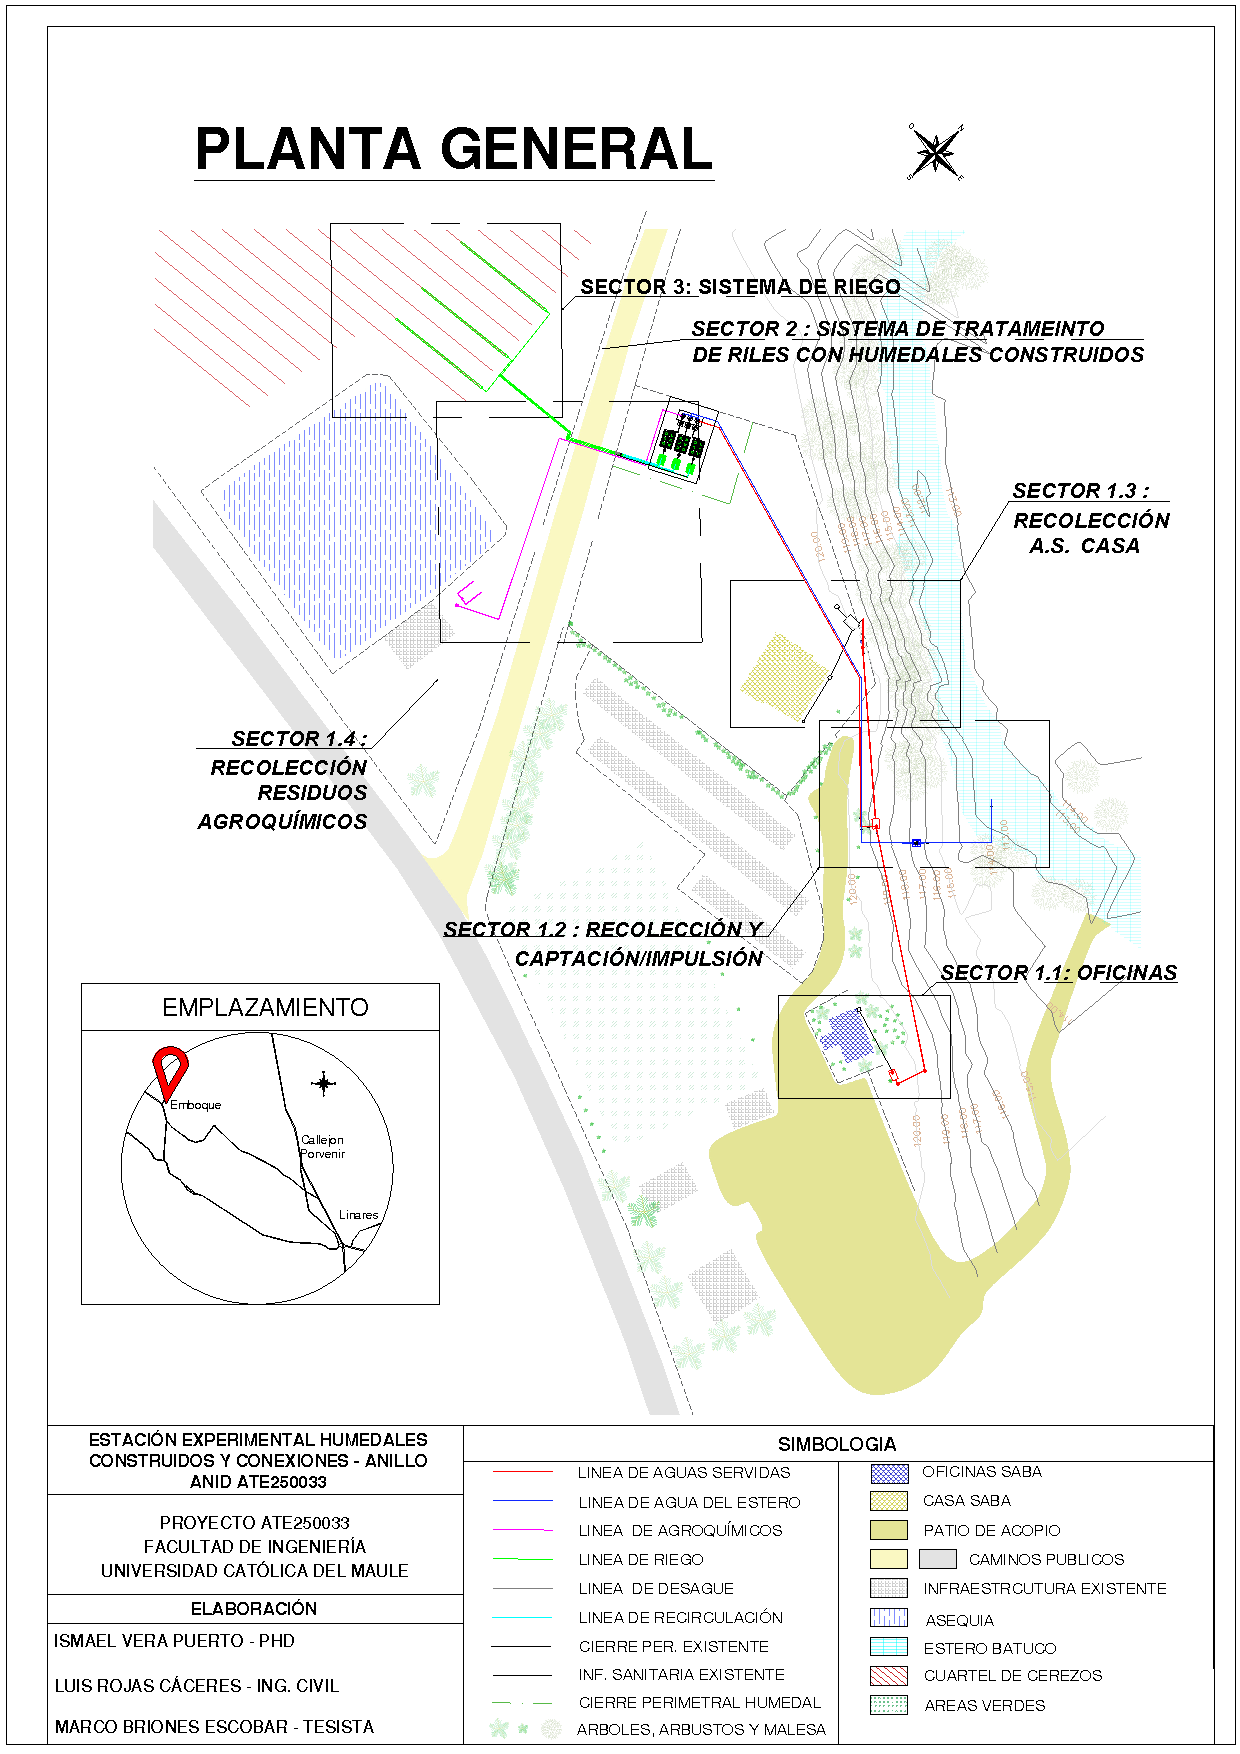
\includegraphics[width=\textwidth, height=0.82\textheight, keepaspectratio]{planos/1_planta-general.pdf}
  \caption{Lámina 1: planta general y de emplazamiento. Fuente: elaboración propia.}
  \label{fig:lamina-1}
\end{figure}

    % Anexo III
% Anexo IV — Planimetría de recolección, impulsión y tratamiento. Origen: v3.0, Anexo D.
\chapter{Planimetría de recolección, impulsión y tratamiento}
\label{anx:planimetria-hidraulica}

Las \cref{fig:lamina-2-1a,fig:lamina-2-1b,fig:lamina-2-2a,fig:lamina-2-2b,fig:lamina-2-3,fig:lamina-2-4} presentan las láminas del sistema hidráulico y de tratamiento.

\begin{figure}[p]
  \centering
  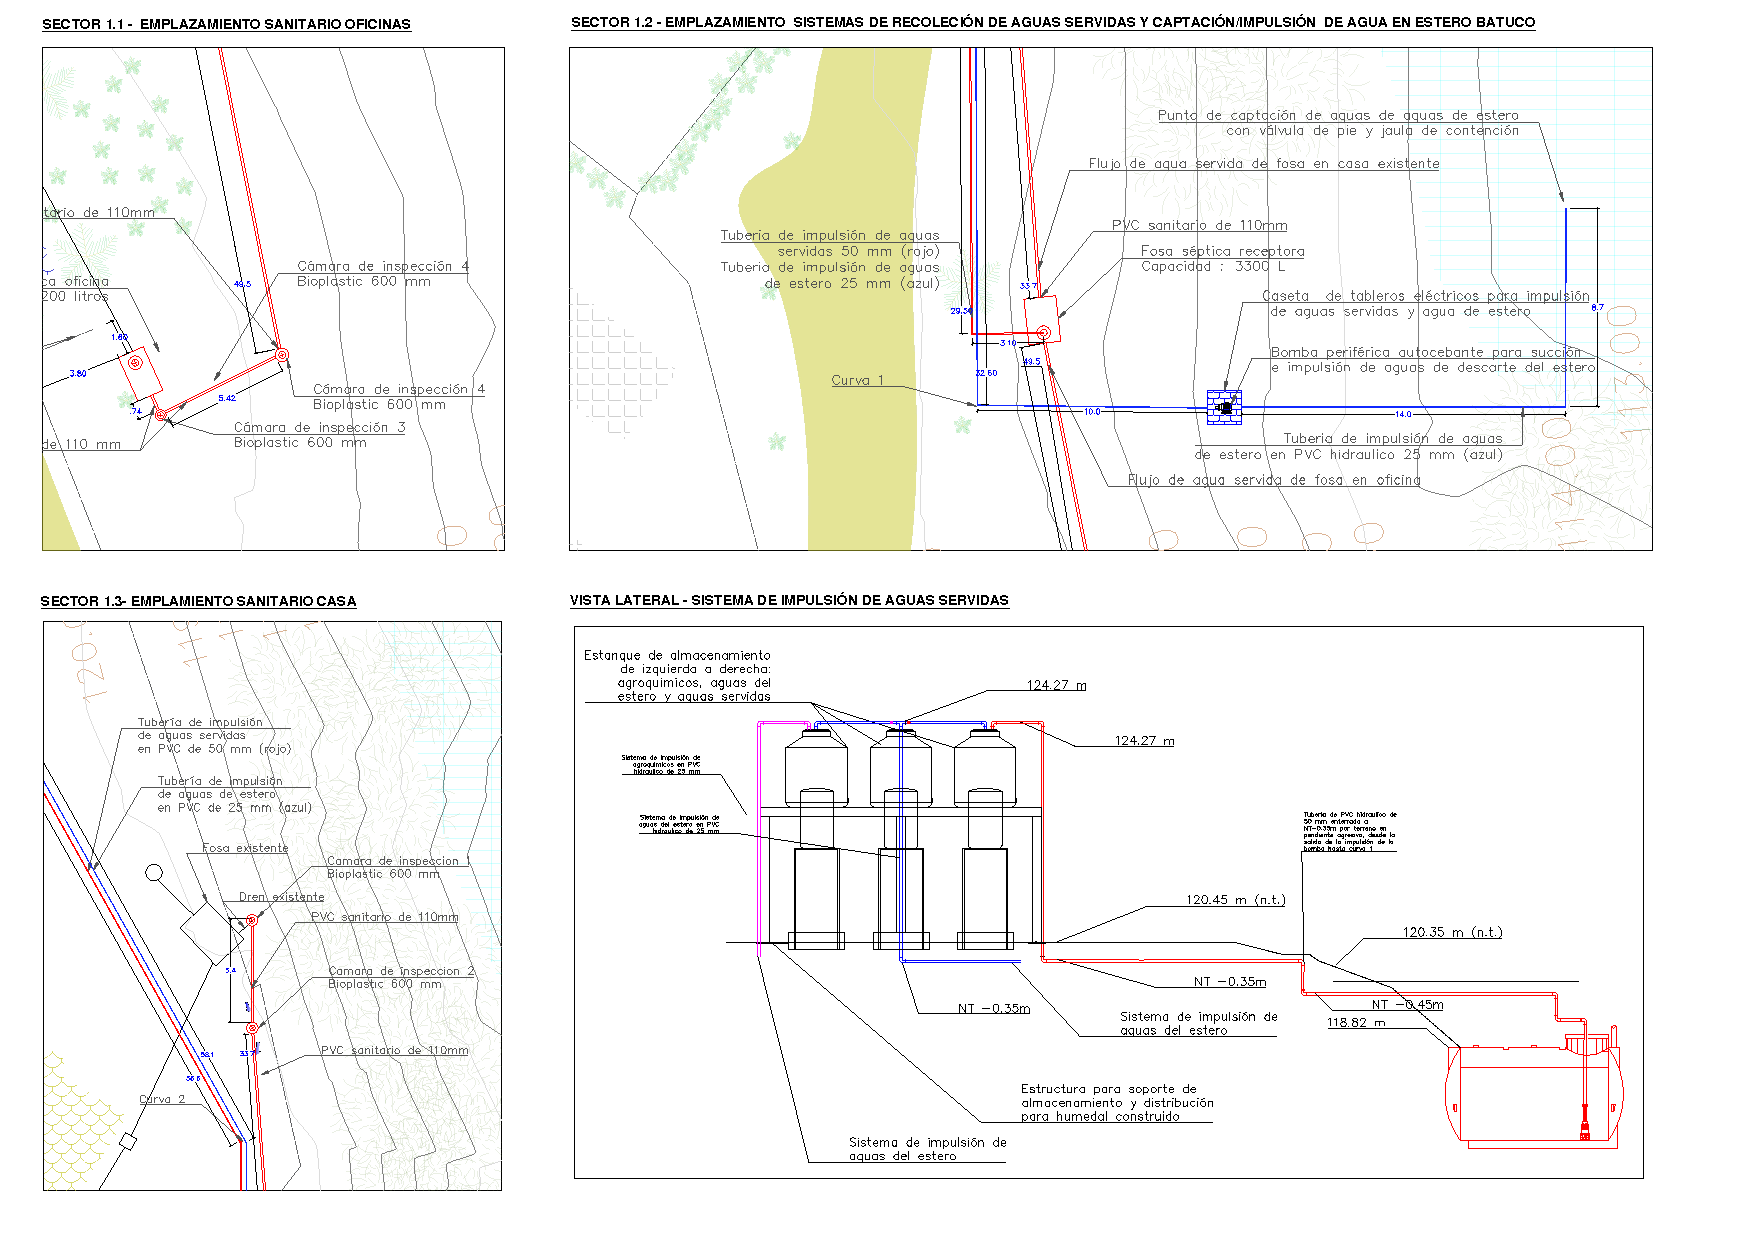
\includegraphics[angle=90, height=0.82\textheight, width=\textwidth, keepaspectratio]{planos/2_1_recoleccion-impulsion-planta.pdf}
  \caption{Lámina 2.1: planta del sistema de recolección e impulsión. Fuente: elaboración propia.}
  \label{fig:lamina-2-1a}
\end{figure}

\begin{figure}[p]
  \centering
  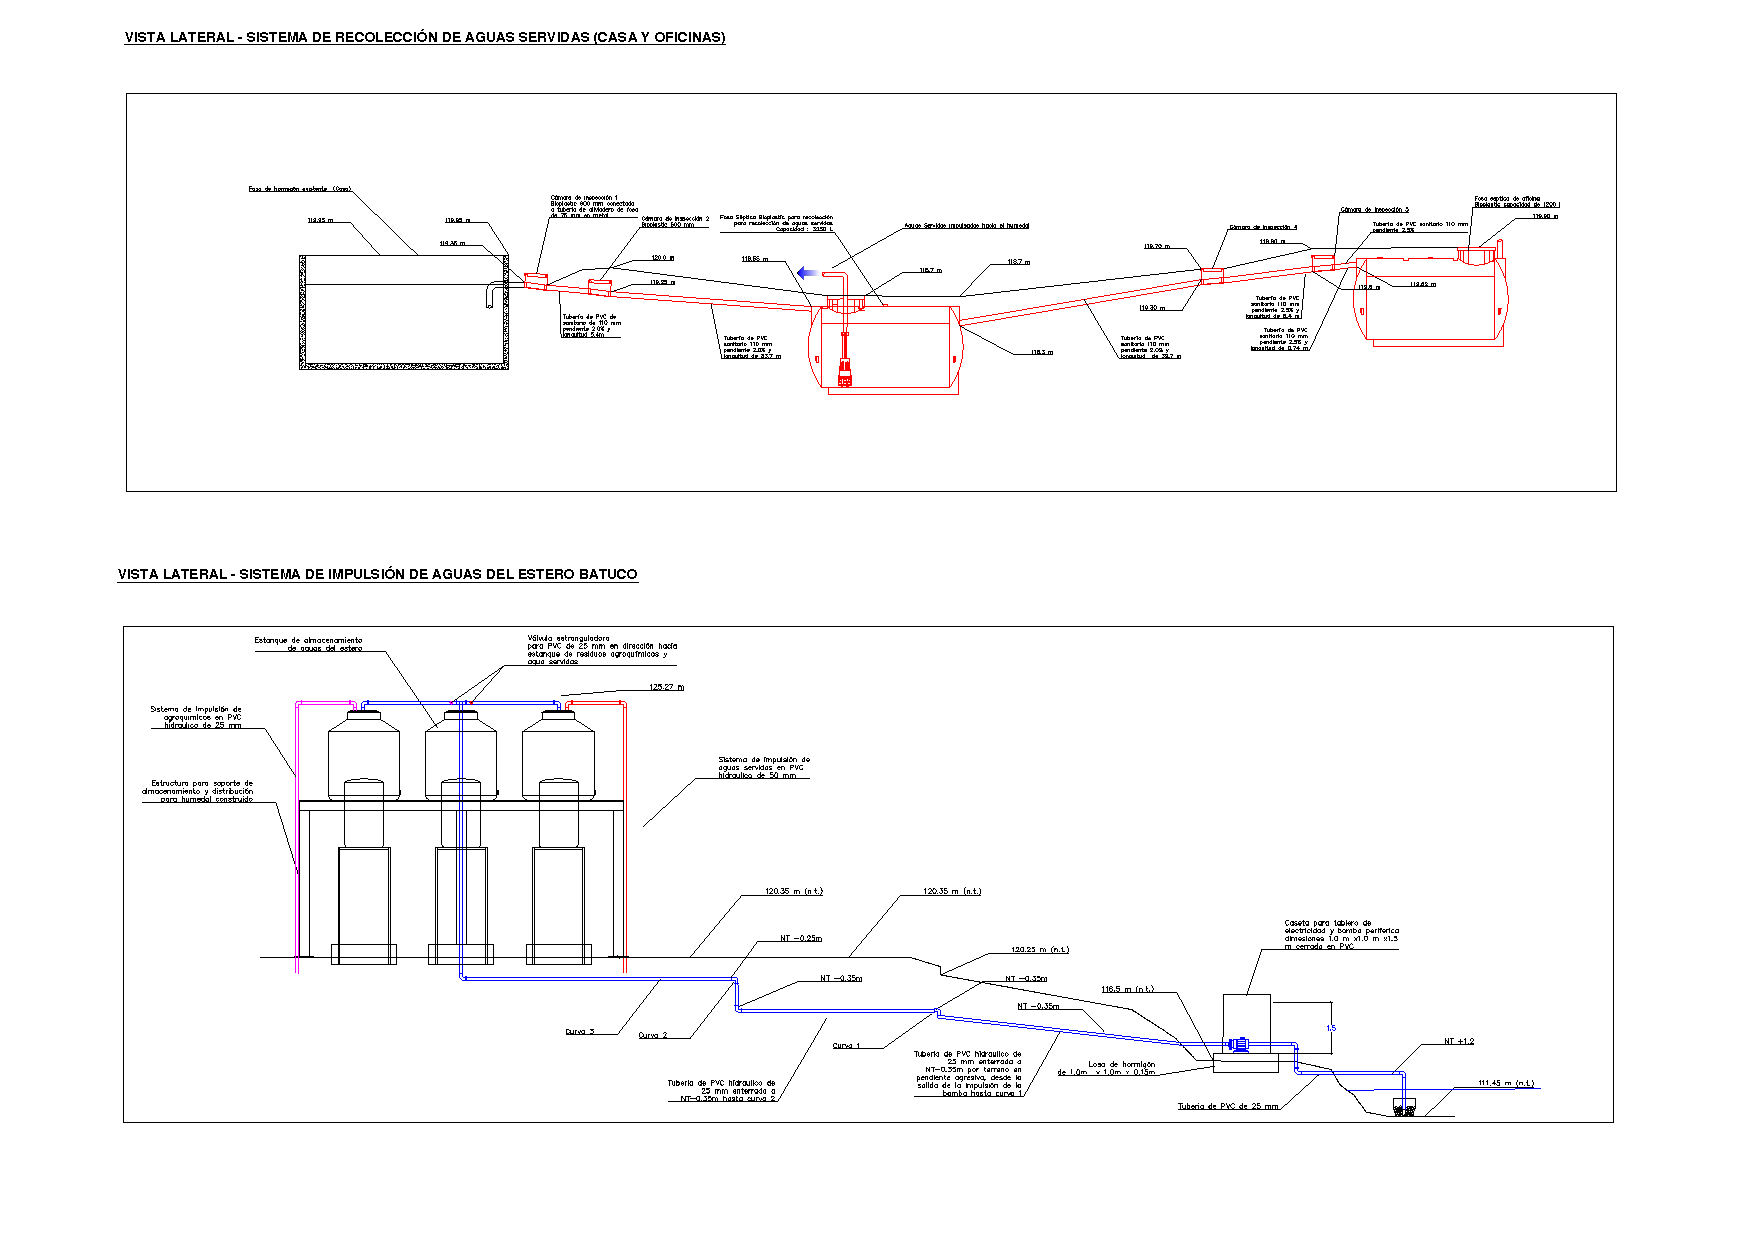
\includegraphics[angle=90, height=0.82\textheight, width=\textwidth, keepaspectratio]{planos/2_1_recoleccion-impulsion-vistas-laterales.pdf}
  \caption{Lámina 2.1: vistas laterales del sistema de recolección e impulsión. Fuente: elaboración propia.}
  \label{fig:lamina-2-1b}
\end{figure}

\begin{figure}[p]
  \centering
  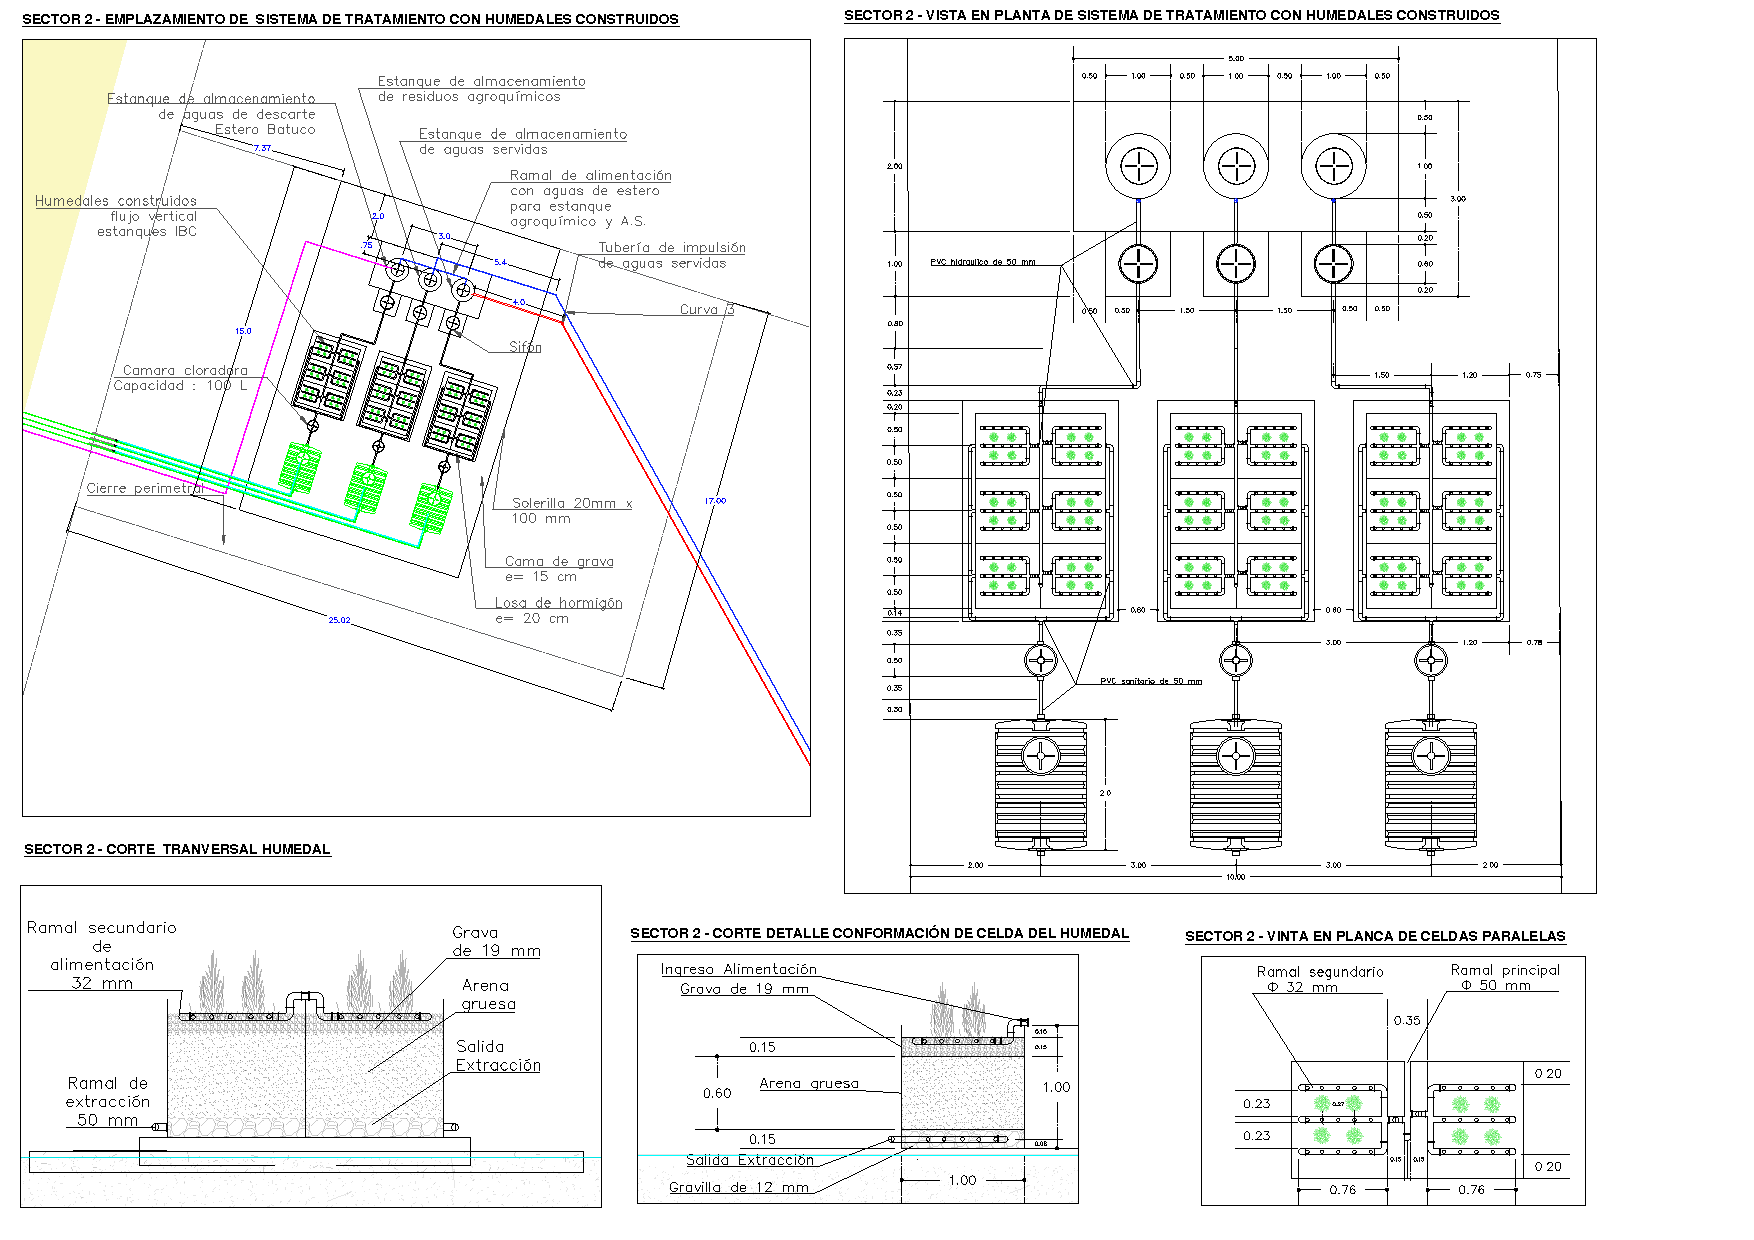
\includegraphics[angle=90, height=0.82\textheight, width=\textwidth, keepaspectratio]{planos/2_2_humedales-planta.pdf}
  \caption{Lámina 2.2: planta general de los humedales construidos. Fuente: elaboración propia.}
  \label{fig:lamina-2-2a}
\end{figure}

\begin{figure}[p]
  \centering
  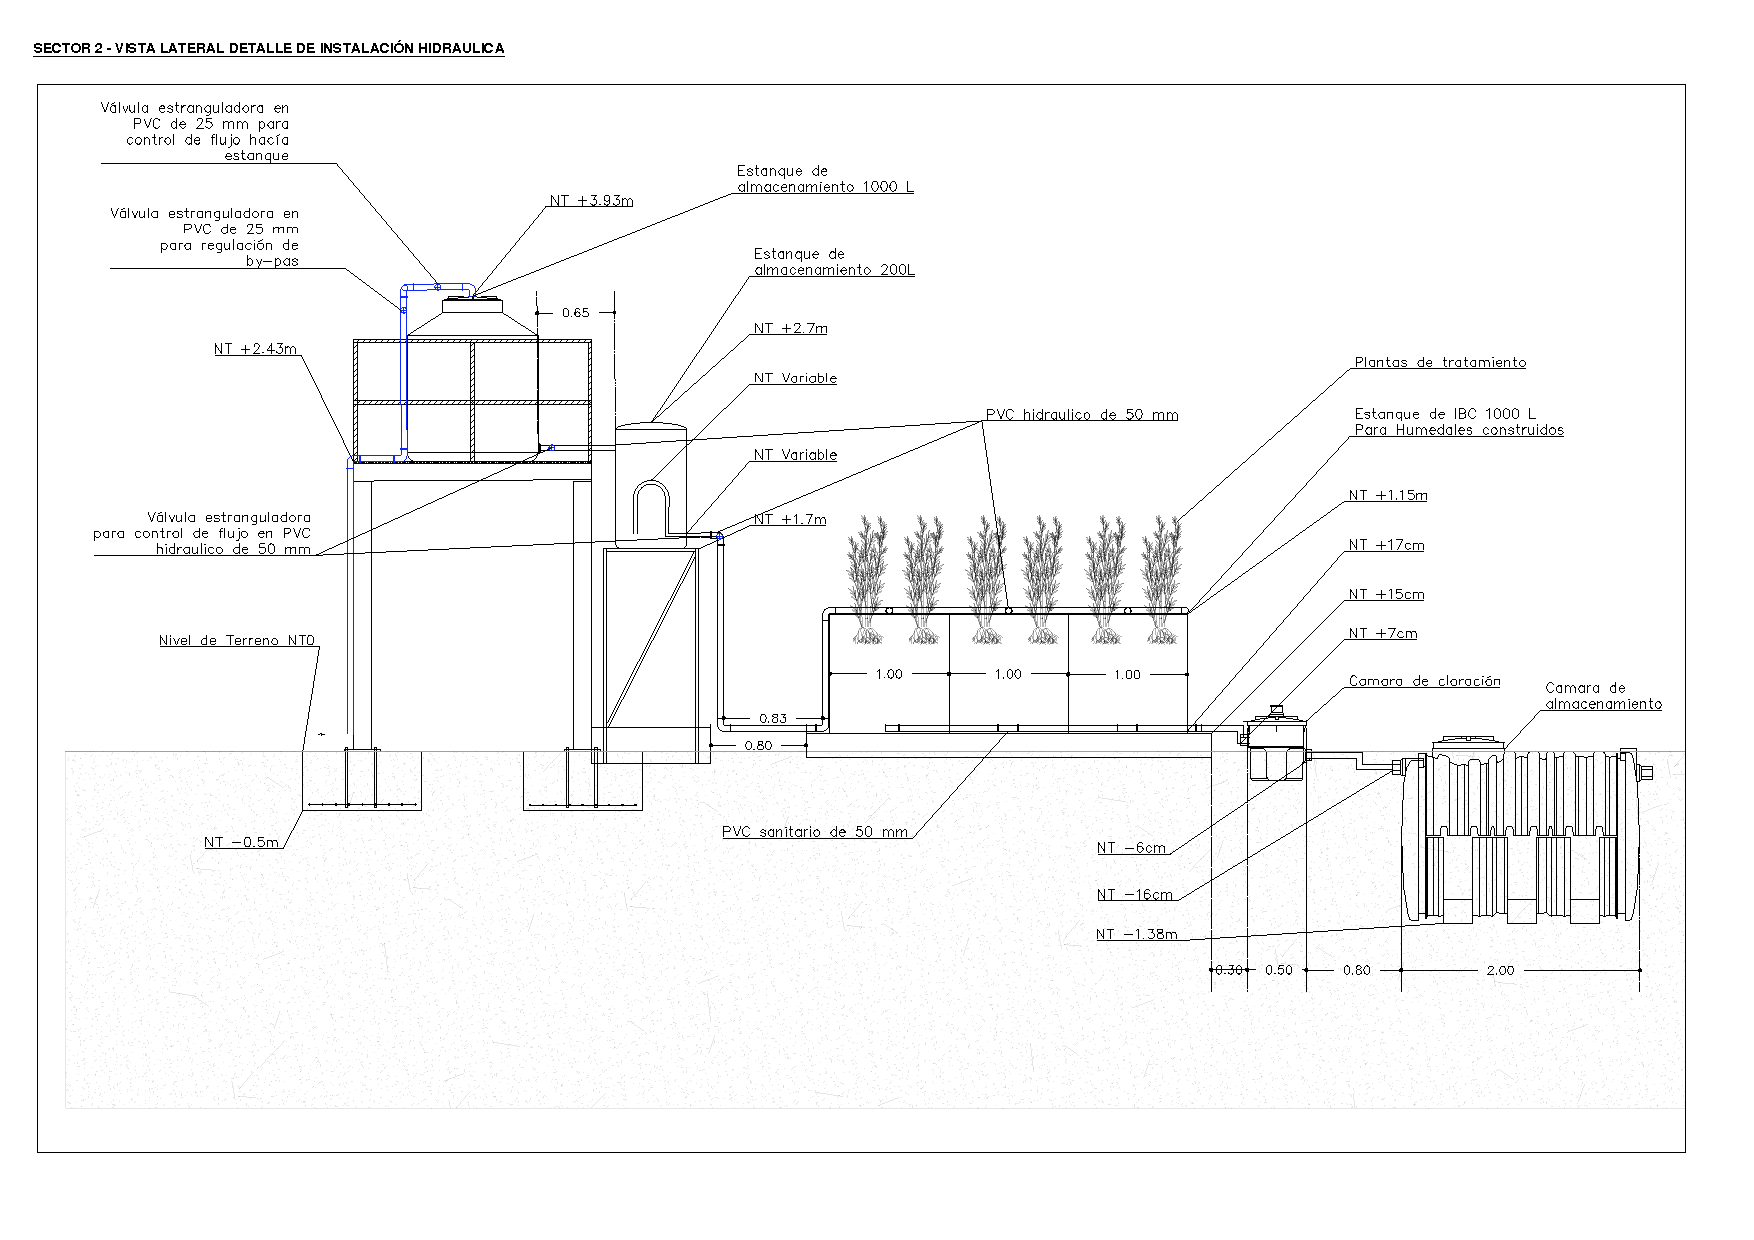
\includegraphics[angle=90, height=0.82\textheight, width=\textwidth, keepaspectratio]{planos/2_2_humedales-vista-lateral.pdf}
  \caption{Lámina 2.2: vista lateral y corte de los humedales construidos. Fuente: elaboración propia.}
  \label{fig:lamina-2-2b}
\end{figure}

\begin{figure}[p]
  \centering
  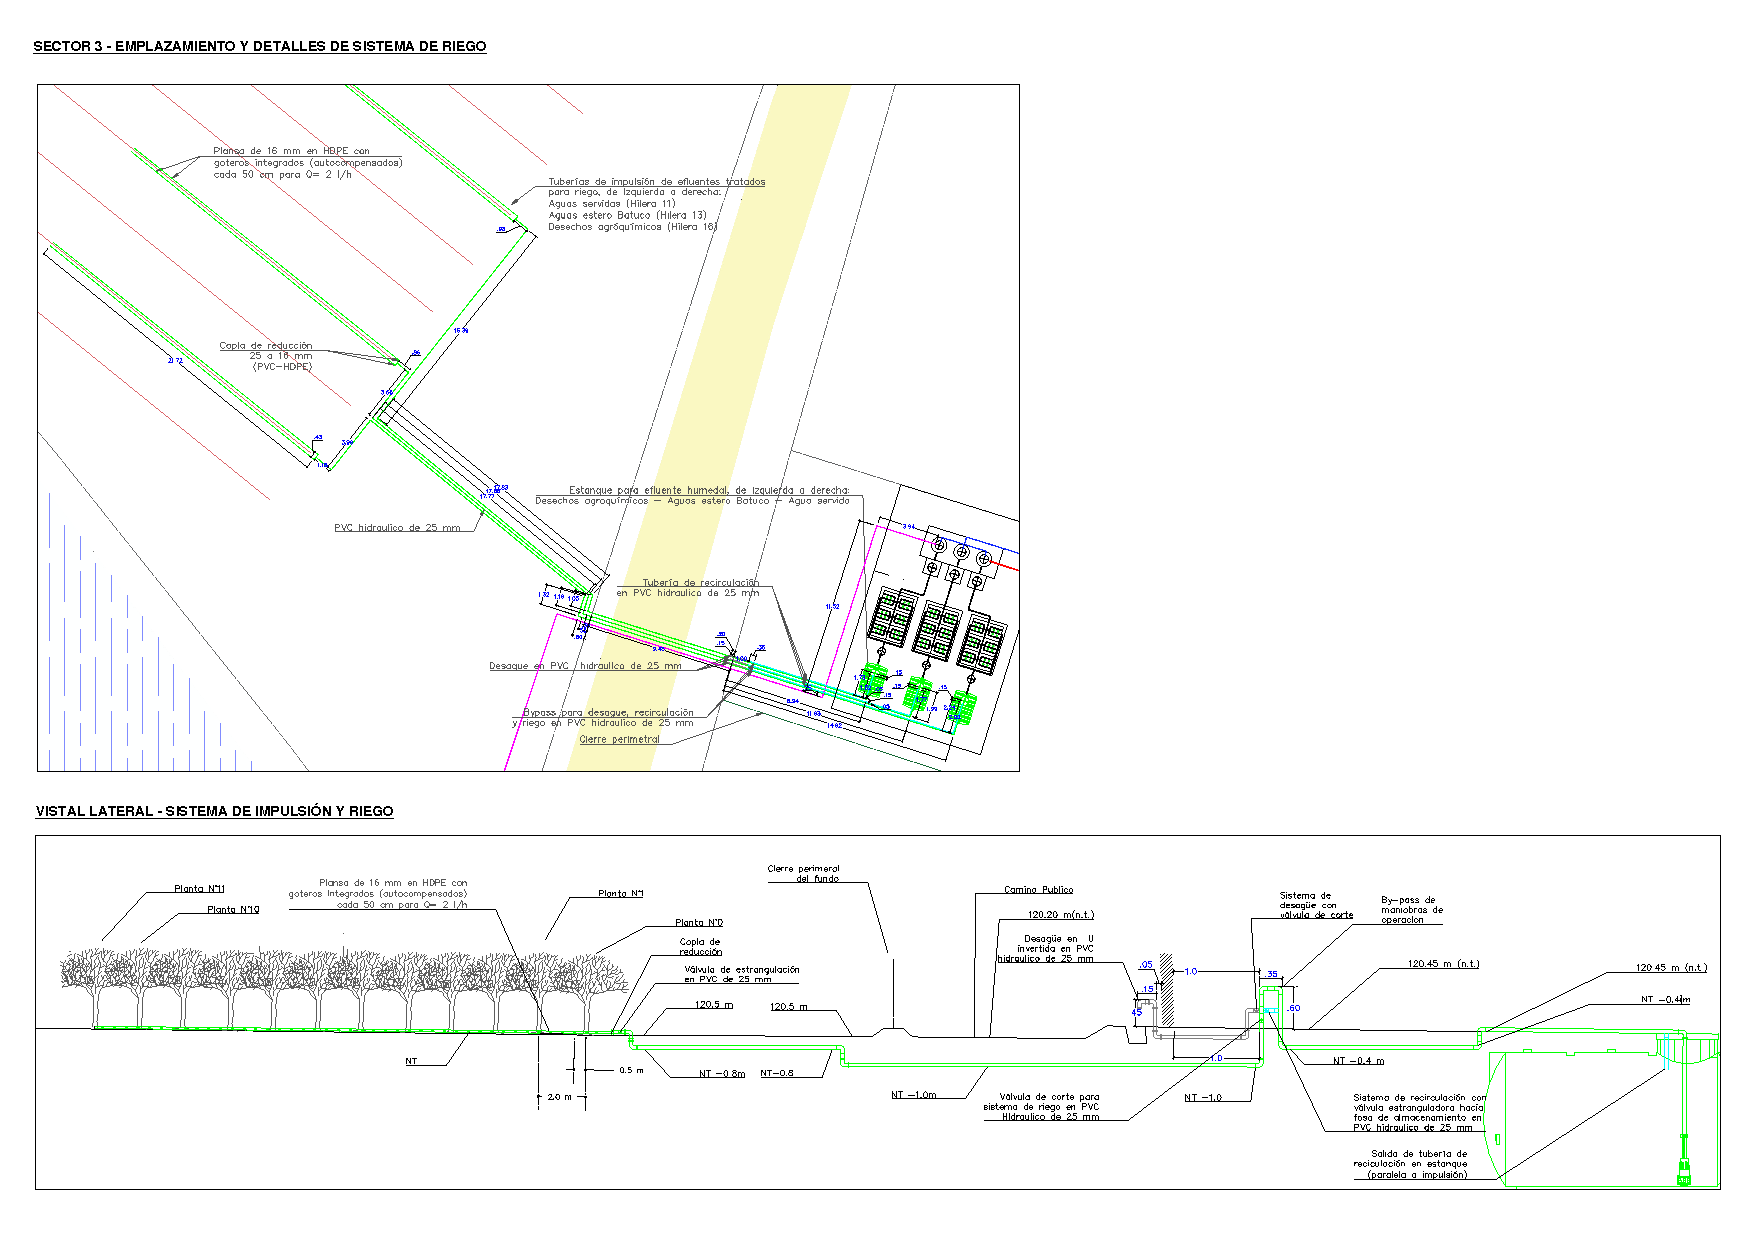
\includegraphics[angle=90, height=0.82\textheight, width=\textwidth, keepaspectratio]{planos/2_3_riego-impulsion.pdf}
  \caption{Lámina 2.3: sistema de riego e impulsión. Fuente: elaboración propia.}
  \label{fig:lamina-2-3}
\end{figure}

\begin{figure}[p]
  \centering
  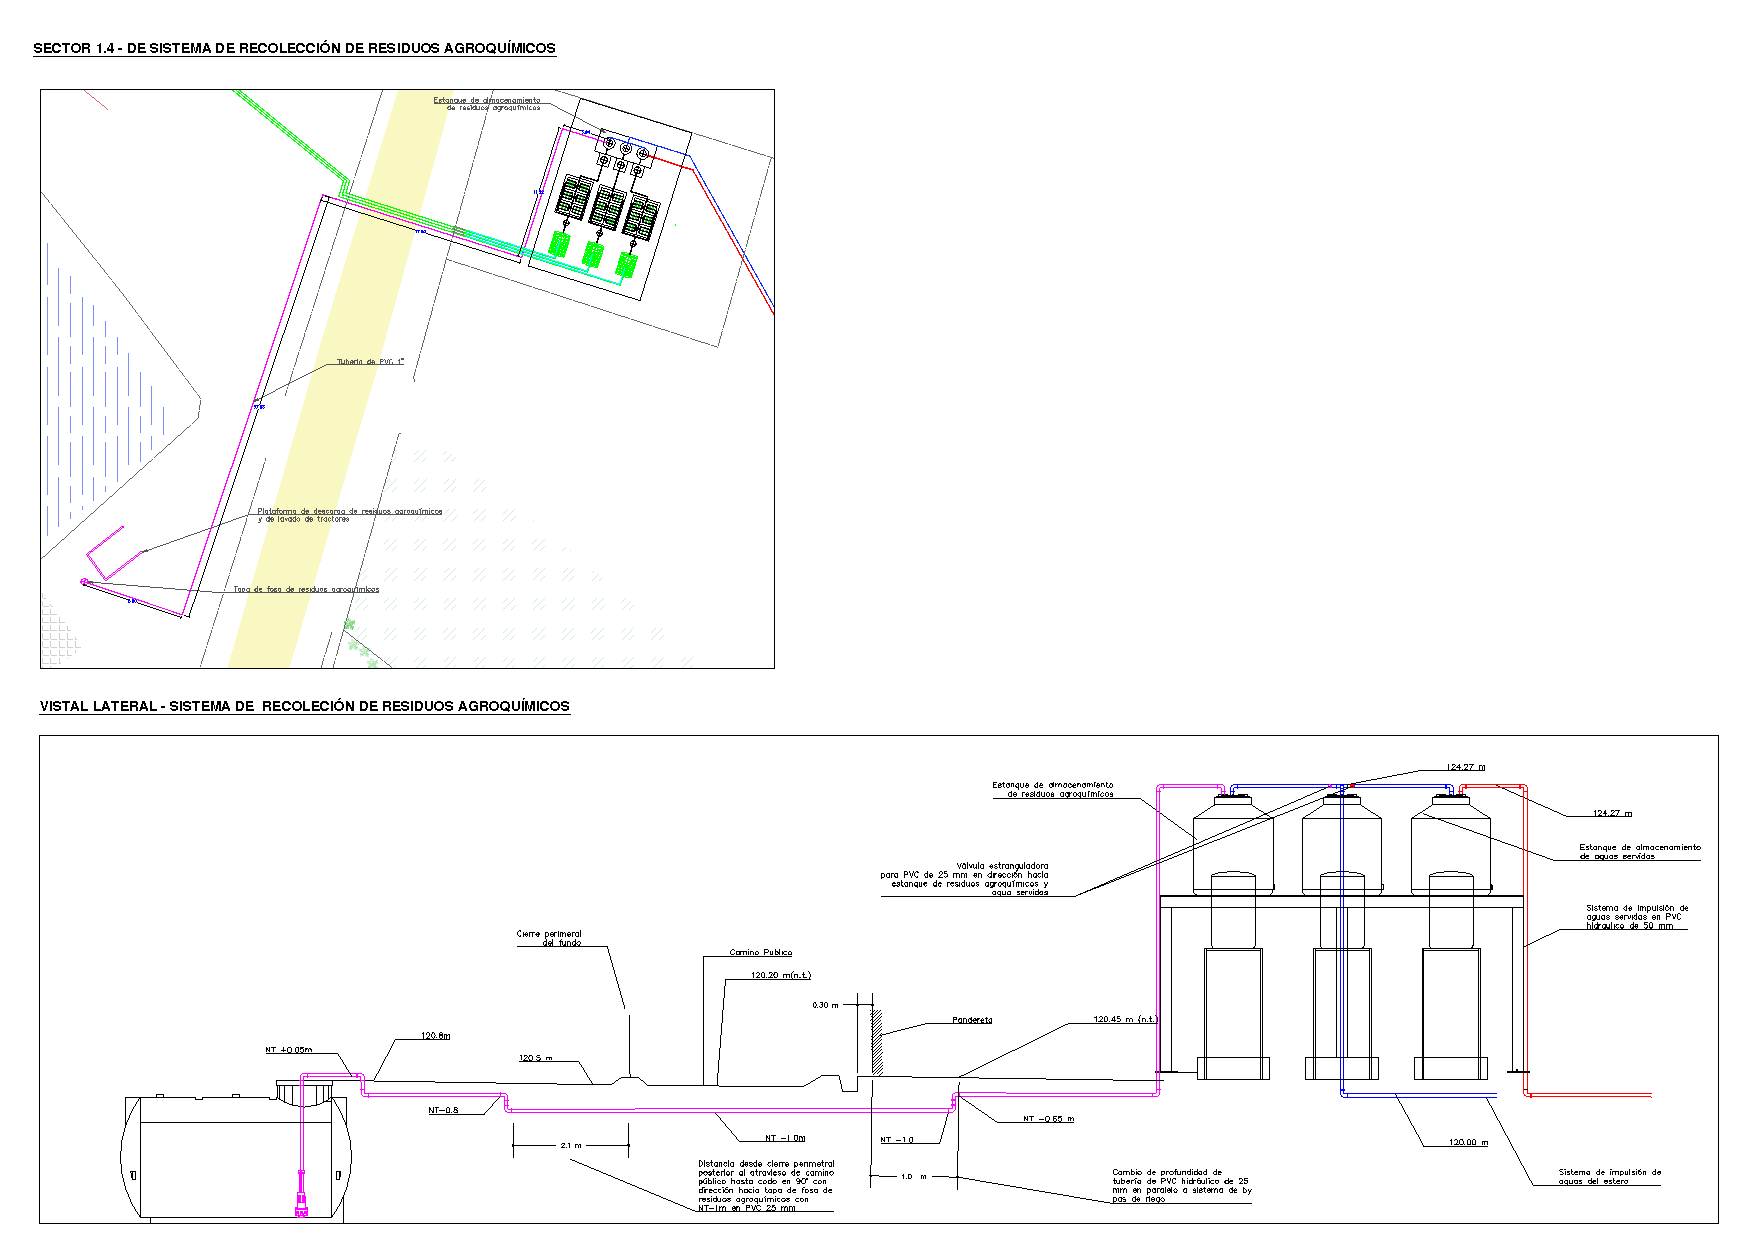
\includegraphics[angle=90, height=0.82\textheight, width=\textwidth, keepaspectratio]{planos/2_4_recoleccion-agroquimicos.pdf}
  \caption{Lámina 2.4: sistema de recolección de residuos agroquímicos. Fuente: elaboración propia.}
  \label{fig:lamina-2-4}
\end{figure}

 % Anexo IV
% Anexo V — Planimetría de detalles estructurales. Origen: láminas 3.1 y 3.2 (PDF vectorial, 2026-11-19).
\chapter{Planimetría de detalles estructurales}
\label{anx:planimetria-estructural}

Las \cref{fig:lamina-3-1,fig:lamina-3-2} presentan los detalles estructurales de la plataforma de soporte de los estanques de almacenamiento.

\begin{figure}[p]
  \centering
  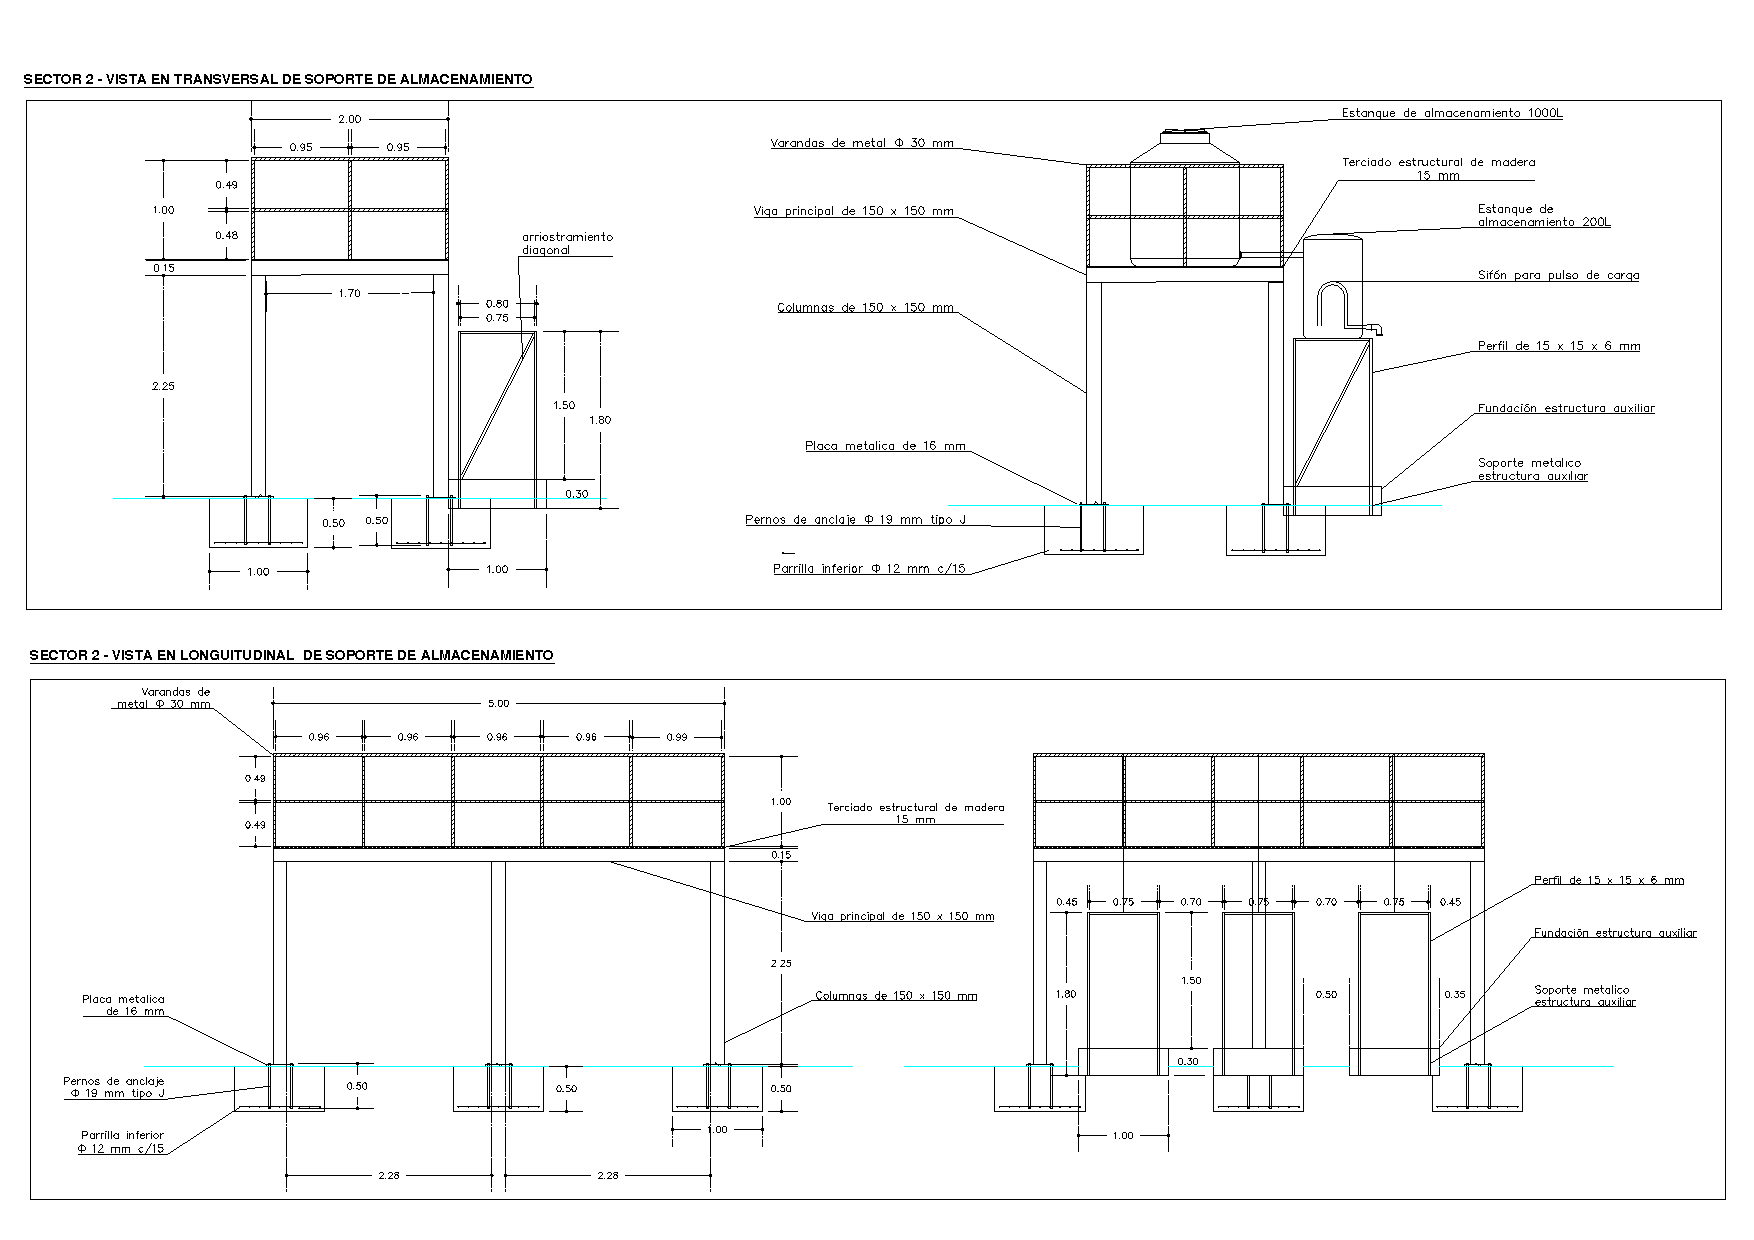
\includegraphics[angle=90, height=0.82\textheight, width=\textwidth, keepaspectratio]{planos/3_1_detalle-estructural-plataforma.pdf}
  \caption{Lámina 3.1: vistas transversal y longitudinal de la estructura de soporte de almacenamiento. Fuente: elaboración propia.}
  \label{fig:lamina-3-1}
\end{figure}

\begin{figure}[p]
  \centering
  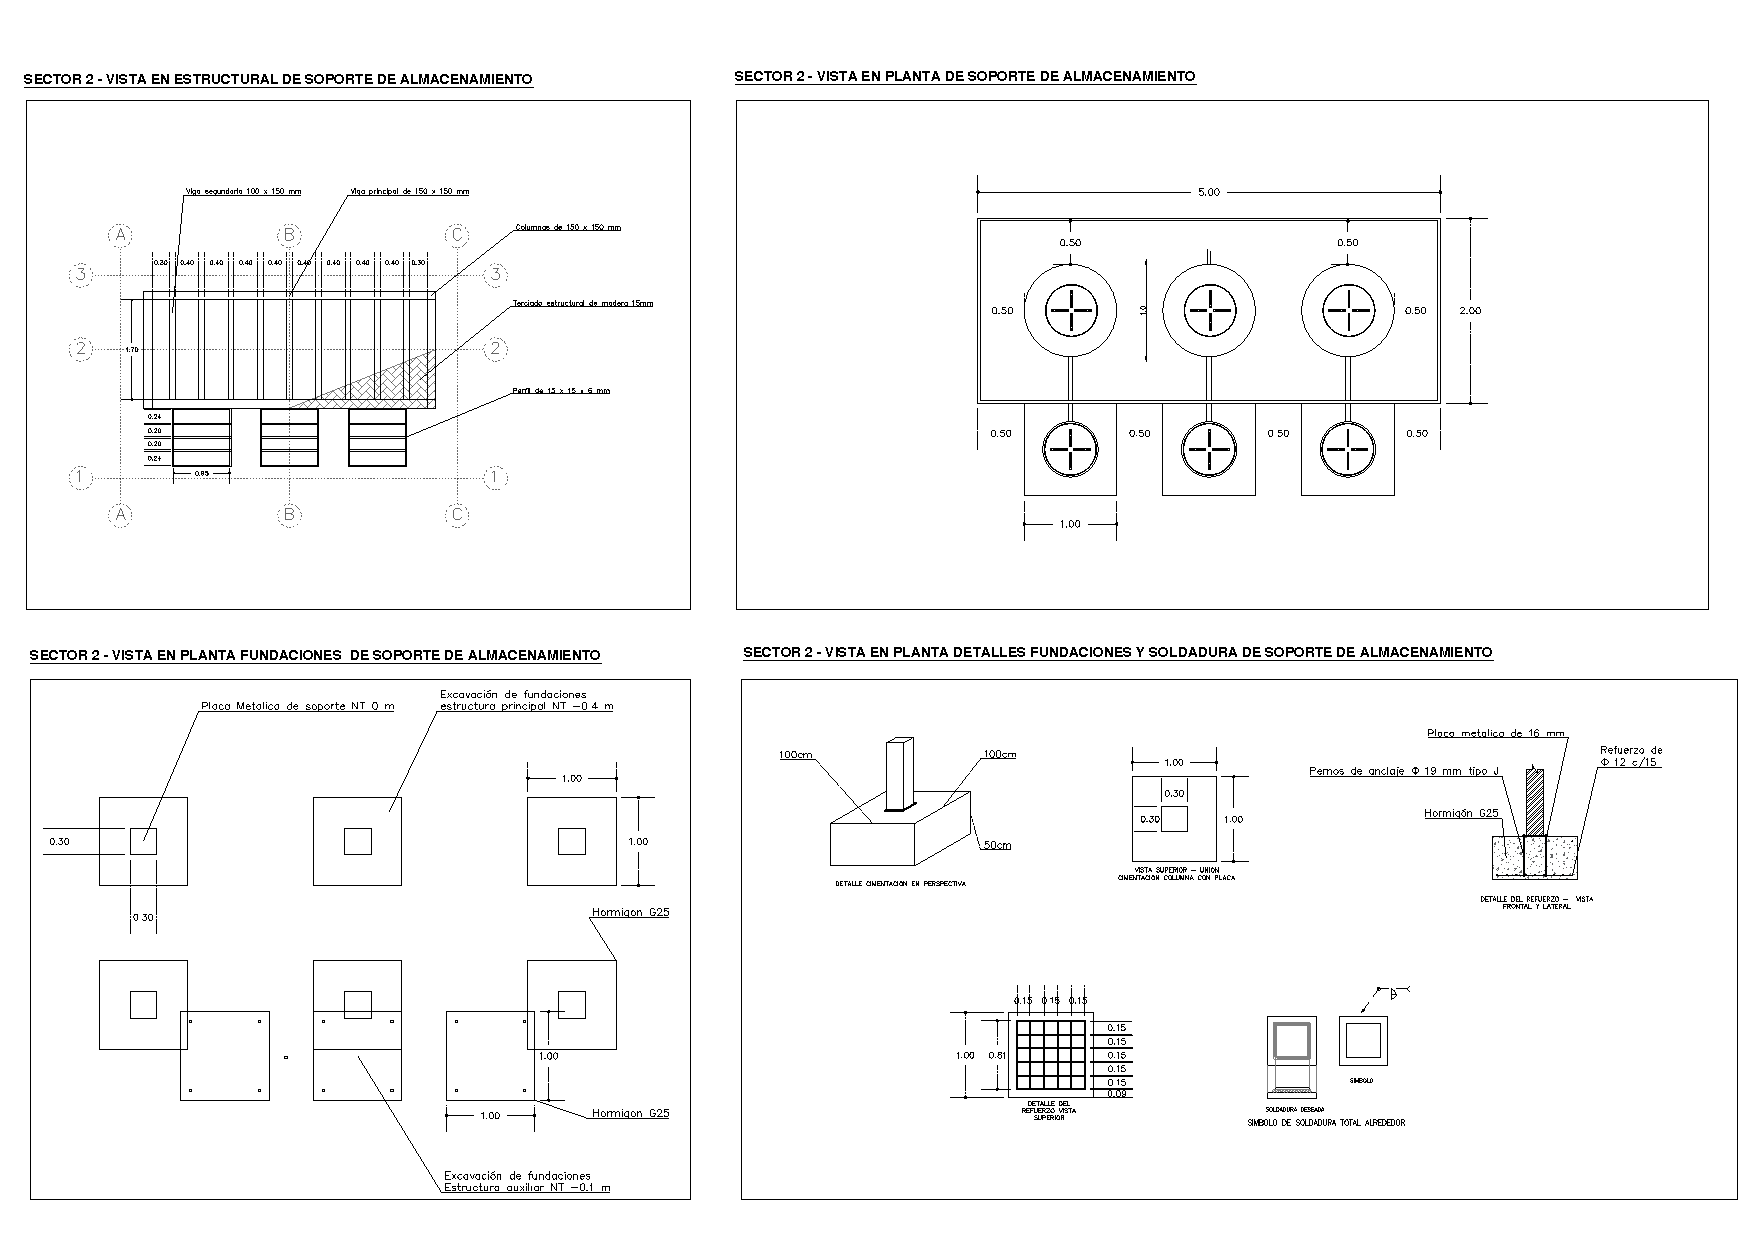
\includegraphics[angle=90, height=0.82\textheight, width=\textwidth, keepaspectratio]{planos/3_2_detalle-estructural-plataforma.pdf}
  \caption{Lámina 3.2: planta estructural, planta de fundaciones y detalles de fundaciones y soldadura. Fuente: elaboración propia.}
  \label{fig:lamina-3-2}
\end{figure}

\revisar{En la lámina 2.4 tengo que corregir la cota de los estanques (\qty{124.27}{\meter} en vez de \qty{125.27}{\meter}), y verificar la profundidad de las fundaciones de la estructura auxiliar (NT $-$\qty{0.1}{\meter} en la lámina 3.2 frente a unos \qty{0.50}{\meter} en la 3.1).}
% Anexo V

\end{document}
